% ****** Start of file aipsamp.tex ******
%
%   This file is part of the AIP files in the AIP distribution for REVTeX 4.
%   Version 4.1 of REVTeX, October 2009
%
%   Copyright (c) 2009 American Institute of Physics.
%
%   See the AIP README file for restrictions and more information.
%
% TeX'ing this file requires that you have AMS-LaTeX 2.0 installed
% as well as the rest of the prerequisites for REVTeX 4.1
%
% It also requires running BibTeX. The commands are as follows:
%
%  1)  latex  aipsamp
%  2)  bibtex aipsamp
%  3)  latex  aipsamp
%  4)  latex  aipsamp
%
% Use this file as a source of example code for your aip document.
% Use the file aiptemplate.tex as a template for your document.
\documentclass[%
 aip,
%jmp,%
%bmf,%
%sd,%
rsi,%
 amsmath,amssymb,
%preprint,%
reprint,%
%author-year,%
%author-numerical,%
]{revtex4-1}

\usepackage{graphicx}% Include figure files
\usepackage{dcolumn}% Align table columns on decimal point
\usepackage{bm}% bold math
%\usepackage[mathlines]{lineno}% Enable numbering of text and display math
%\linenumbers\relax % Commence numbering lines

\usepackage[T1]{fontenc}
\usepackage[utf8]{inputenc}
\usepackage[polutonikogreek,english]{babel}
\usepackage{hyperref}
\hypersetup{colorlinks=true,allcolors=blue}
\usepackage[all]{hypcap}

\newcommand{\micron}{\textgreek{μ}m}
\newcommand{\microsec}{\textgreek{μ}s}
\newcommand{{\usalex}}{\textgreek{μ}sALEX}

\begin{document}

\preprint{AIP/123-QED}

\title[48-spot smFRET-PAX setup]{48-spot single-molecule FRET setup with periodic acceptor excitation}

\author{Antonino Ingargiola}%
\email{ingargiola.antonino@gmail.com}
\author{Maya Segal}
\affiliation{
Dept. Chemistry and Biochemistry, University of California Los Angeles, USA}
\author{Angelo Gulinatti}
\author{Ivan Rech}
\author{Ivan Labanca}
\affiliation{%
DEIB, Politecnico di Milano, Italy
}%
\author{Piera Maccagnani}
\affiliation{Istituto per la Microelettronica e Microsistemi, IMM-CNR, Bologna, Italy.}
\author{Massimo Ghioni}
\affiliation{%
DEIB, Politecnico di Milano, Italy
}%
\author{Shimon Weiss}%
\author{Xavier Michalet}%
 \email{michalet@chem.ucla.edu}
\affiliation{
Dept. Chemistry and Biochemistry, University of California Los Angeles, USA}


\date{\today}% It is always \today, today,
             %  but any date may be explicitly specified

\begin{abstract}
Single-molecule FRET (smFRET) allows measuring distances between donor (D) and
acceptor (A) fluorophores on the 3-10~nm range.
Solution-based smFRET allows measurement of binding-unbinding events
or conformational changes of dye-labeled biomolecules without ensemble averaging
and free from surface perturbations. When employing dual (or multi)
laser excitation,
smFRET allows resolving the number of fluorescent
labels on each molecule, greatly enhancing the ability to study
heterogeneous samples.
A major drawback to solution-based smFRET is the low throughput,
which renders repetitive measurements expensive and hinders the ability
to study kinetic phenomena in real-time.

Here we demonstrate a high-throughput smFRET system which
multiplexes acquisition by using 48 excitation spots and two
48-pixel SPAD array detectors. The system employs two excitation lasers
allowing separation of species with one or two active fluorophores.
The performance of the system is demonstrated on a set of doubly-labeled
double-stranded DNA oligonucleotides
with different distances between D and A dyes along the DNA duplex.
We show that the acquisition time for accurate subpopulation identification
is reduced from several minutes to seconds, opening the way
to high-throughput screening applications and
real-time kinetics studies of enzymatic reactions such as DNA transcription
by bacterial RNA polymerase.
\end{abstract}

\keywords{Single-molecule FRET, high-throughput, SPAD array}
%Use showkeys class option if keyword display desired
\maketitle

\section{Introduction} \label{sec:intro}

Detailed knowledge of the three-dimensional (3D) atomistic structure of
macromolecular complexes is essential to understand their
biological function. For decades, X-ray crystallography and nuclear
magnetic resonance (NMR) spectroscopy have been the techniques of choice
for obtaining atomically resolved macromolecular structures. More recently,
single-particle cryo-electron microscopy (cryo-EM) has complemented these
methods for determination of large macromolecular structures with the
added ability to classify different conformations. However, macromolecules
spontaneously and dynamically explore various conformations in equilibrium
that are hard to capture by the above-mentioned methods. Understanding the
functional roles of these structures requires a full dynamic picture.
Single-molecule Förster resonance energy transfer (smFRET) paved the way
for studying such structural dynamics in biologically-relevant conditions.
smFRET allows determination of each conformational state that may exist in
the ensemble of macromolecular complexes as well as the distance between
specific residues for each
state~\cite{dahan_ratiometric_1999,deniz_single-pair_1999,ha_single-molecule_1999,kapanidis_fluorescence-aided_2004}.
Recently, several groups used smFRET to
measure distances between multiple distinct pairs of residues to
construct 3D macromolecular structures of distinct conformations by
triangulation and comparison to existing X-ray crystal
structures~\cite{dimura_quantitative_2016,hellenkamp_multidomain_2017,hoefling_structural_2011,kalinin_toolkit_2012,muschielok_nano-positioning_2008,muschielok_application_2011}.
Moreover, smFRET can measure the evolution in time of multiple
distances between multiple FRET pairs, and hence report upon the dynamic
3D structure of a macromolecule undergoing conformational changes.
So far, however, due to the requirement of low sample concentration imposed
by the necessity to have no more than one molecule within the
diffraction-limited confocal volume at a given
time~\cite{dahan_ratiometric_1999,fries_quantitative_1998},
only very slow kinetics could be measured. Therefore, increased throughput
is essential for both static and dynamic measurements of multiple distances.

To overcome
this limitation, we recently introduced a multispot excitation scheme taking
advantage of novel single-photon avalanche diode (SPAD)
arrays~\cite{ingargiola_parallel_2012,ingargiola_8-spot_2013,ingargiola_multispot_2017}.
We demonstrated that the resulting setup indeed allows acquisition of
single-molecule data comparable to that of standard single-spot
setups, but with a throughput that scales with the number
of excitation spots.
We illustrated an application of this enhanced throughput
by measuring the bubble closing kinetics during promoter escape in bacterial
transcription~\cite{ingargiola_multispot_2017}.
While encouraging, these results were partially unsatisfactory because they
were obtained with a rather small number of spots (8), and also because
the setup only incorporated a single laser, used for excitation of the
donor (D) dye of the FRET donor-acceptor (D-A) pair~\cite{ingargiola_multispot_2017}.
Single-laser smFRET is unable to distinguish between low FRET molecules
(molecules with two active D and A dyes in which the D-A distance is
large compared to the characteristic FRET length scale) from D-only molecules
(i.e. molecules with a single D dye, or dually-labeled molecules
with an inactivated or bleached A dye).
Since the latter categories are present in most samples,
it is important to identify and separate them from low FRET molecules
of interest.

To address this problem, \emph{Microsecond Alternated Laser EXcitation}
smFRET (referred throughout as {\usalex} for brevity), was
introduced several years ago~\cite{kapanidis_alternating-laser_2005},
and later extended to pulsed laser excitation schemes
(nsALEX~\cite{laurence_probing_2005} or PIE~\cite{muller_pulsed_2005}).
Briefly, in {\usalex},
two exciting lasers are alternatively turned on and off every few tens of
{\microsec} allowing the separation of species with only a single active
dye (D-only, A-only populations) from doubly-labeled species with both dyes
active (FRET population). In fact, only for FRET populations, there
is a fluorescence signal both during the D-laser excitation (due to
excitation of the D dye) and the A-laser excitation (due to excitation
of the A dye).
This, in turn, extends the number of FRET sub-populations that can be possibly
identified within a sample in the regime of low mean FRET efficiencies.
This scheme has since been extended to 3 or 4 laser excitations, allowing
powerful molecular sorting applications~\cite{lee_three-color_2007,yim_four-color_2012}.
A simplified version of this laser alternation principle was presented in
ref.~\onlinecite{doose_periodic_2007}, where the D-excitation laser
is left on at all times while the A-laser is alternated.
This Periodic Acceptor Excitation single-molecule FRET
technique~\cite{doose_periodic_2007} (referred to as PAX for brevity) allows
simplifying
the optical setup while maintaining the advantages of {\usalex}, namely
the ability to determine the stoichiometry of D and A dyes on each single molecule
or to identify changes in the fluorescence quantum yields~\cite{lee_accurate_2005}.
Here we present a significant improvement to our original multispot
setup by (i) introducing a 48-spot illumination and detection scheme,
and (ii) implementing a 2-laser PAX illumination approach.

Software needed to operate the multispot setup (including
LCOS-SLM pattern generation, LabVIEW-FPGA timestamping code,
piezo-motor control, etc.) is organized in different repositories
and available on GitHub at
\href{https://github.com/multispot-software}{https://github.com/multispot-software}.

This paper is organized as follows.
In section~\ref{sec:setup_brief} we briefly introduce the optical setup,
the detectors (section~\ref{sec:detectors}) and the modulation scheme
(section~\ref{sec:48spot-pattern}). In section~\ref{sec:smfret-meas} we
report single-molecule measurements, starting with a brief
description of the data analysis (section~\ref{sec:analysis}).
To demonstrate the uniformity across channels, for each spot we report
the peak photon rate in bursts (section~\ref{sec:peak-phrate})
and E-S histograms (section~\ref{sec:EShist}).
Finally, in section~\ref{sec:alexpax-comp} we present a
comparison of single-spot {\usalex} and 48-spot PAX measurements
for a 15~second acquisition.

\begin{figure*}
    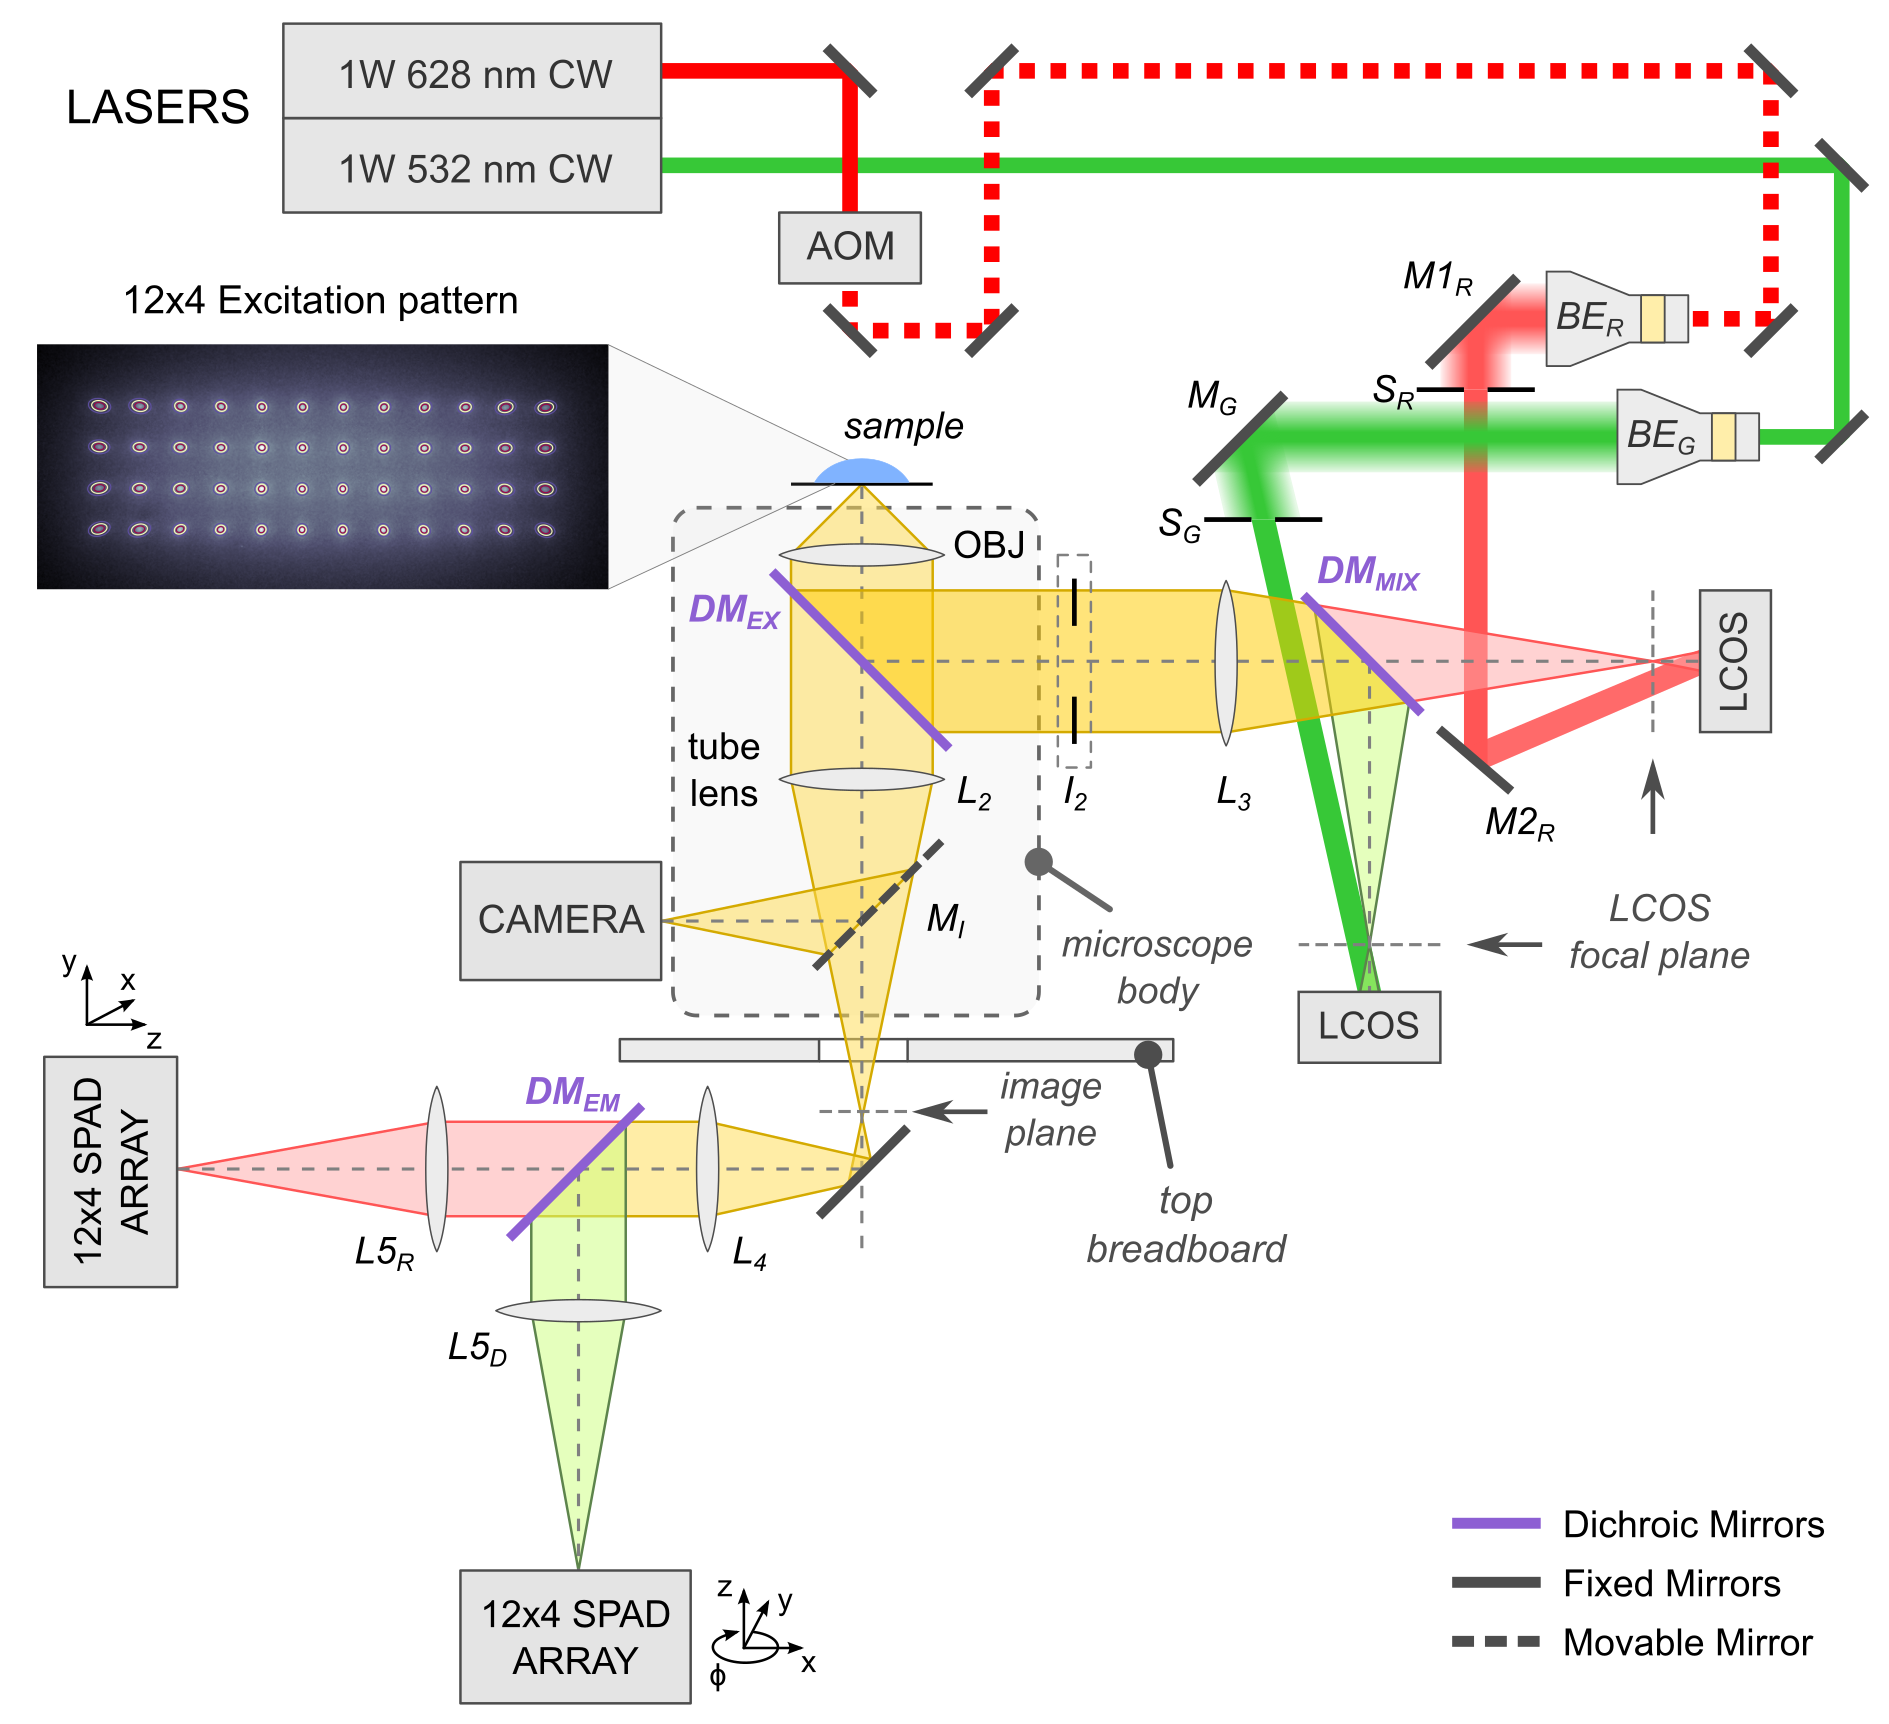
\includegraphics[width=0.7\textwidth]{figures/design_multispot_LCOS_camera_SPAD}
    \caption{{\label{fig:setup} Schematic of the 48-spot smFRET-PAX setup. See
    man text and appendix~\ref{sec:setup} for a detailed description.}}
\end{figure*}

\section{Setup description}
\label{sec:setup_brief}

In this section, we outline a brief description of the setup.
A more detailed description can be found in
appendix~\ref{sec:setup}, while details of laser and SPAD array
alignment can be found in appendix~\ref{sec:laseralign}
and~\ref{sec:spadalign} respectively.

A schematic of the setup is reported in Fig.~\ref{fig:setup}.
The setup includes two 1W CW excitation laser (green: 532~nm, red: 628~nm)
with only the red laser being modulated via an acoustic-optic modulator (AOM).
After polarization adjustment and beam expansion, the two lasers
are phase modulated by the respective LCOS-SLM generating two
48-spots patterns on a plane after each LCOS-SLM (\emph{LCOS image plane}).
The two lasers are then combined by a dichroic mirror ($DM_{MIX}$) and
recollimated ($L_3$) before being focused into the sample by an
high numerical aperture (NA) objective lens (60x, NA=1.2).
Emitted fluorescence is collected by the same objective lens,
separated by excitation wavelength through a dual-band polychroic mirror ($DM_{EX}$),
and focused by a tube lens ($L_2$) into the image plane.
Next, emitted fluorescence light is recollimated ($L_4$), separated into donor
and acceptor spectral bands ($DM_{EM}$), and focused into two different
48-pixel SPAD arrays that are mounted on motorized micro-positioning stages.
The system is aligned so that each SPAD pixel is optically
conjugated to one excitation spot into the sample.

Output from the detectors is processed by an FPGA-based board which performs
photon timestamping with 12.5~ns resolution and transfers data to a
host PC.
The host PC runs an acquisition software that displays 96-channel timetraces
in real-time, implements alignment routines, and saves the acquisition to
disk. Further data conversion and analysis is performed on a second PC.

\subsection{Detectors}
\label{sec:detectors}

The current 48-spot setup employs two identical 12x4-pixel SPAD arrays whose
architecture and performance has been presented
in~\onlinecite{gulinatti_48-pixel_2013}.
Here we describe only the most salient features.
The active area of each pixel has a 50~{\micron}
diameter. The array is comprised by 4 rows of 12 pixels (4x12) with a
500~{\micron} pitch in each direction.

To easily integrate the detectors into a multispot setup,
we developed a photon-counting module that integrates a 48-pixel SPAD
array and the electronics required for device operation, data acquisition,
and transmission into a compact, user friendly module.
In particular, the SPAD array is housed into a hermetically
sealed chamber separated from the rest of the module. Sealing in a dry
atmosphere makes it possible to mount the array on a double-stage Peltier,
cooling the detector down to temperatures of approximately $-15^{\circ}$C and
thereby reducing the dark count rate (DCR) and increasing the sensitivity of the
instrument. Photon-counting pulses are made externally available through a standard
SCSI connector. This allows for an easy connection of the module to
general-purpose boards for data acquisition and processing.
Alternatively, an onboard FPGA (Spartan 6 SLX150, Xilinx, San Jose, CA, USA)
can be used to time-stamp counts detected in each of the 48-channels
with a time resolution of 10~ns where this information is sent
to a remote PC through a high-speed USB link.
A C-mount at the top of the photon-counting module
allows for easy and reliable connections to the multispot setup.

The two SPAD arrays used in the current 48-spot smFRET-PAX setup are operated
at a temperature of -10 $^{\circ}$C.
The photon detection efficiency (PDE) reaches a maximum of $\sim$45\%
at 550~nm and drops to 35\% at
628nm\cite{gulinatti_48-pixel_2013,michalet_silicon_2014}. The PDE is highly
uniform over the array, with a peak-to-peak spread of only a few percent.
Fig.~\ref{fig:dcr} shows heatmaps of dark count rates for the two
12x4 SPAD arrays. About 80\% of the pixels have a DCR lower than 1000 counts
per second (cps), whereas the worst performing pixel has
a fairly low DCR of less than 6~kcps.

48-spot smFRET-PAX results were compared to the state-of-the-art single-spot
{\usalex} setup previously described in~\onlinecite{ingargiola_multispot_2017}.
This setup employs two single-pixel commercial SPADs
(SPCM-AQRH, Excelitas Technology Corp., Waltham, MA, USA)
characterized by PDE similar to our SPAD arrays in the D spectral band
but with a more than two-fold higher PDE in the A spectral band.
For this reason, the {\usalex} setup is expected to be
at least twice as sensitive in the A-channel than the 48-spot setup.
A detailed comparison of the different SPAD technologies for single-molecule
measurements is reported in~\onlinecite{michalet_silicon_2014}.

\begin{figure}
    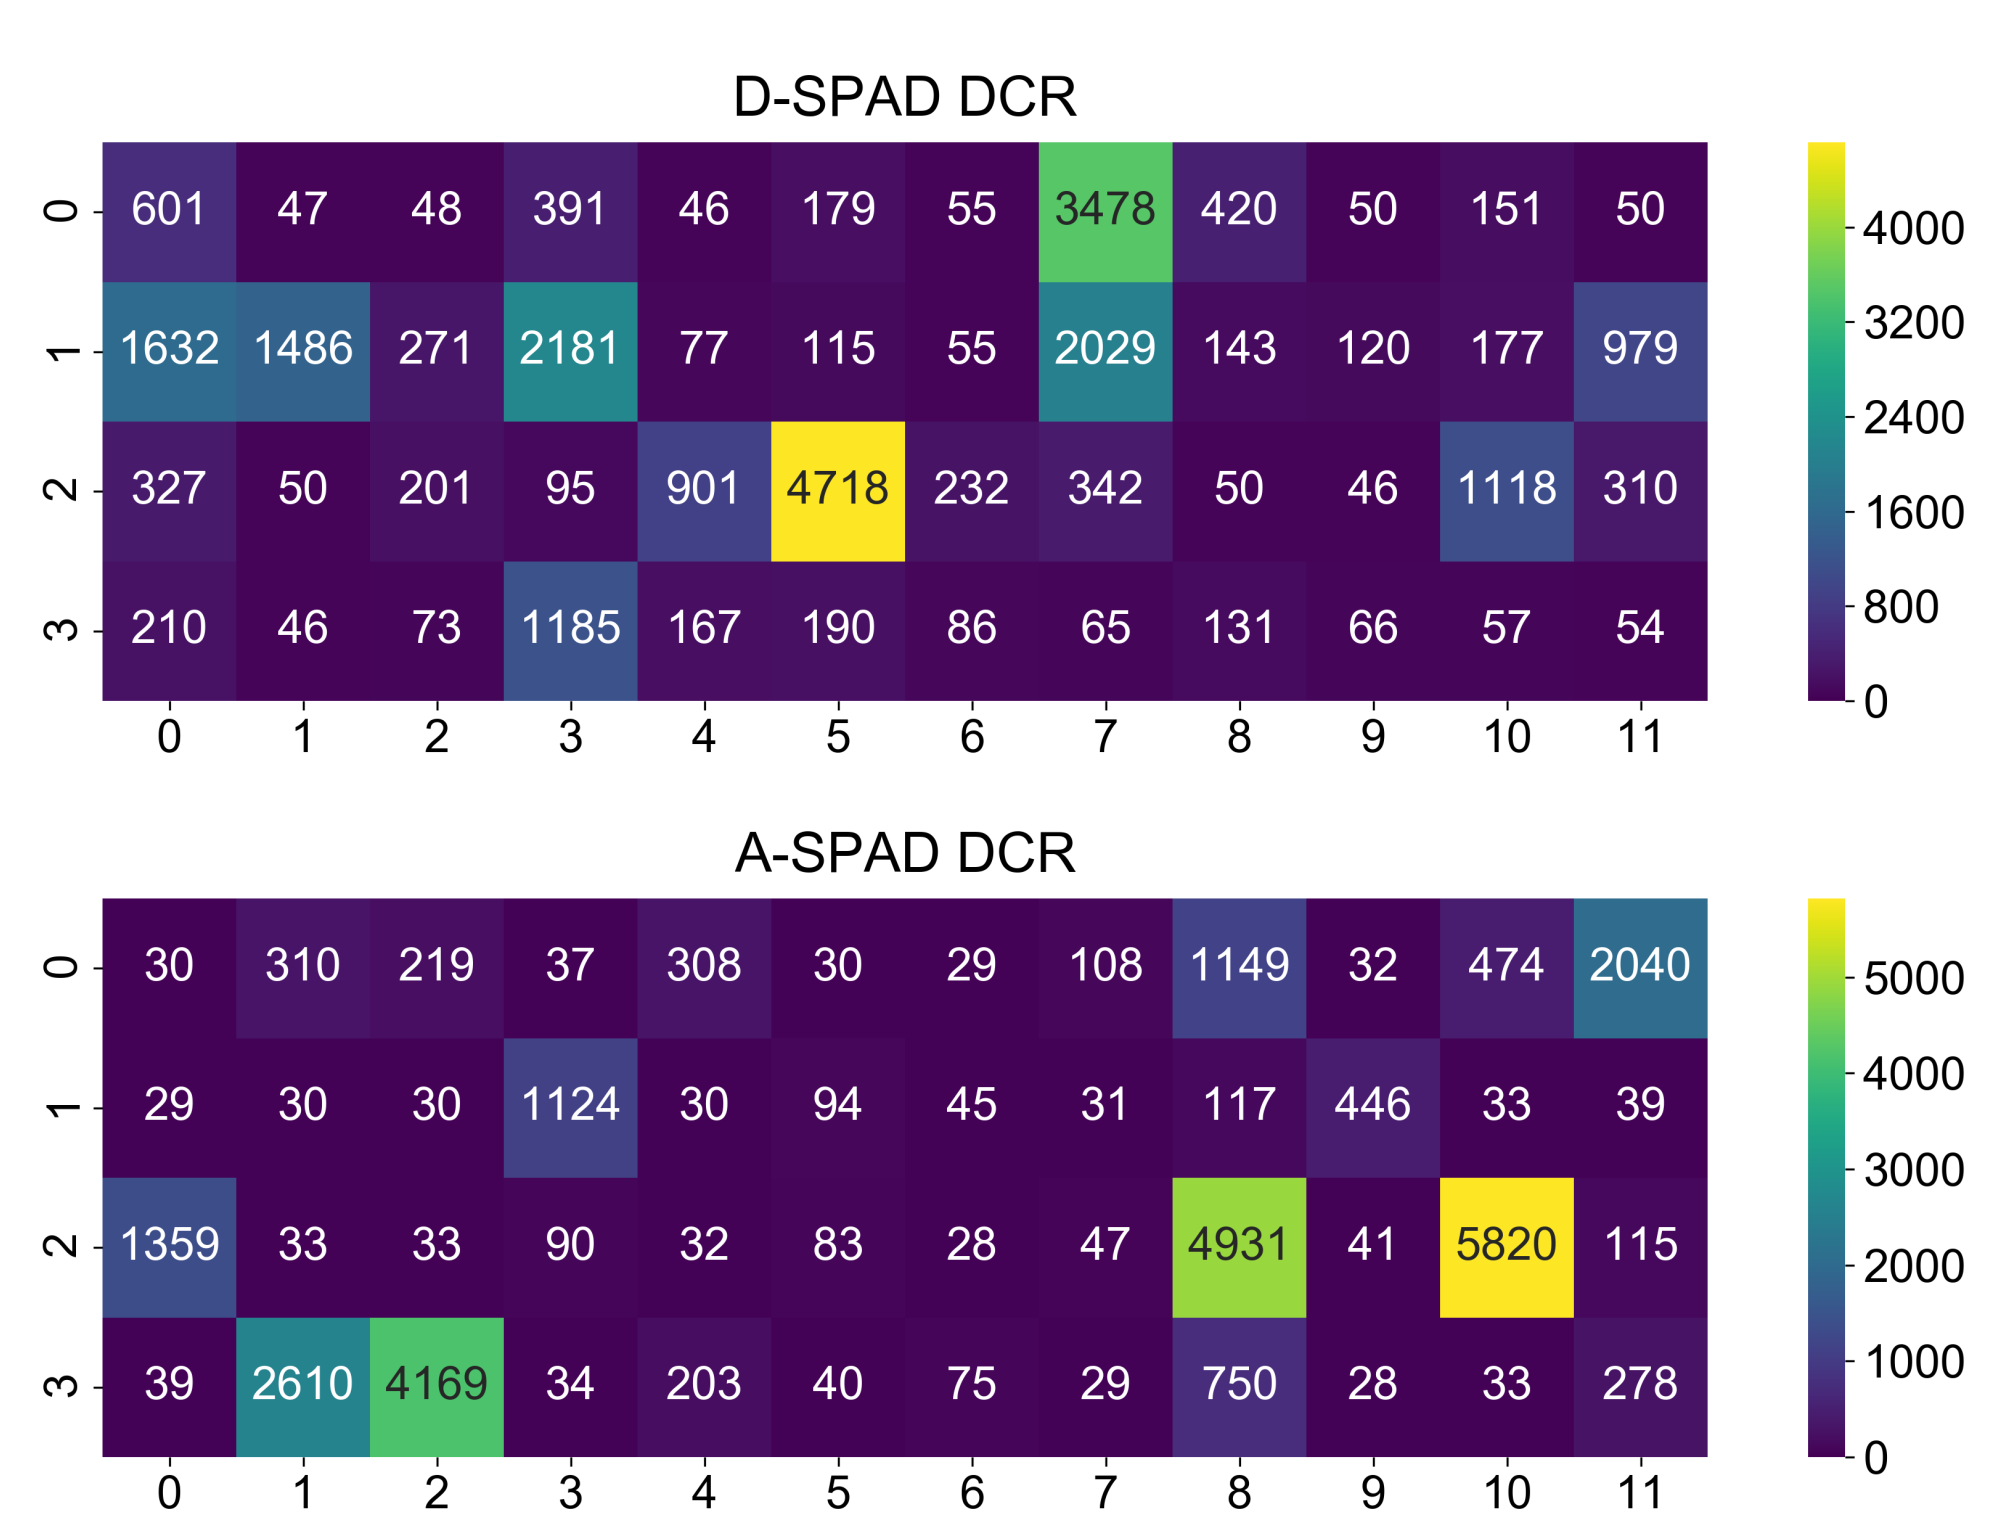
\includegraphics[width=\columnwidth]{figures/DCR-comp}
    \caption{{\label{fig:dcr} Heatmaps of dark count rates (DCR) for the 12x4
    D and A SPAD arrays used in the current 48-spot smFRET-PAX setup.
    DCR values are overlaid on each pixel. All values are in counts per second (cps).
    More details and data underlying this figure can be found in the
    \href{https://github.com/48-spot-paper-analysis}{48-spot-paper-analysis}.}}
\end{figure}

\subsection{48-spot pattern}
\label{sec:48spot-pattern}

The 48 excitation spots are generated independently for each wavelength by
phase modulation of an incoming plane wave, as previously described
in~\onlinecite{colyer_high-throughput_2010,ingargiola_multispot_2017}. The
phase modulation operates in direct space rather than Fourier space and
implements the phase profile of a Fresnel lenslet array. Delon's groups
employed a conceptually similar direct-space modulation  scheme using an
LCOS-SLM for multi-confocal fluorescence correlation  spectroscopy
(FCS)~\cite{kloster-landsberg_cellular_2012} (although they use a different
spatial arrangement of the phase pattern on the LCOS-SLM).

Fig.~\ref{fig:patternfit} shows the emission pattern due to the green (Panel A)
and red lasers (Panel B) acquired by a camera on the microscope side-port
using a high-concentration dye sample. The two patterns are aligned to
maximize overlap of each of the 48 spots.
Overlap of the two wavelengths and centering with respect to
the optical axis is assessed via 2-D Gaussian fitting as reported in Panel C.
Full details on the alignment procedure and pattern assessment
can be found in appendix~\ref{sec:lcos}.

\begin{figure}
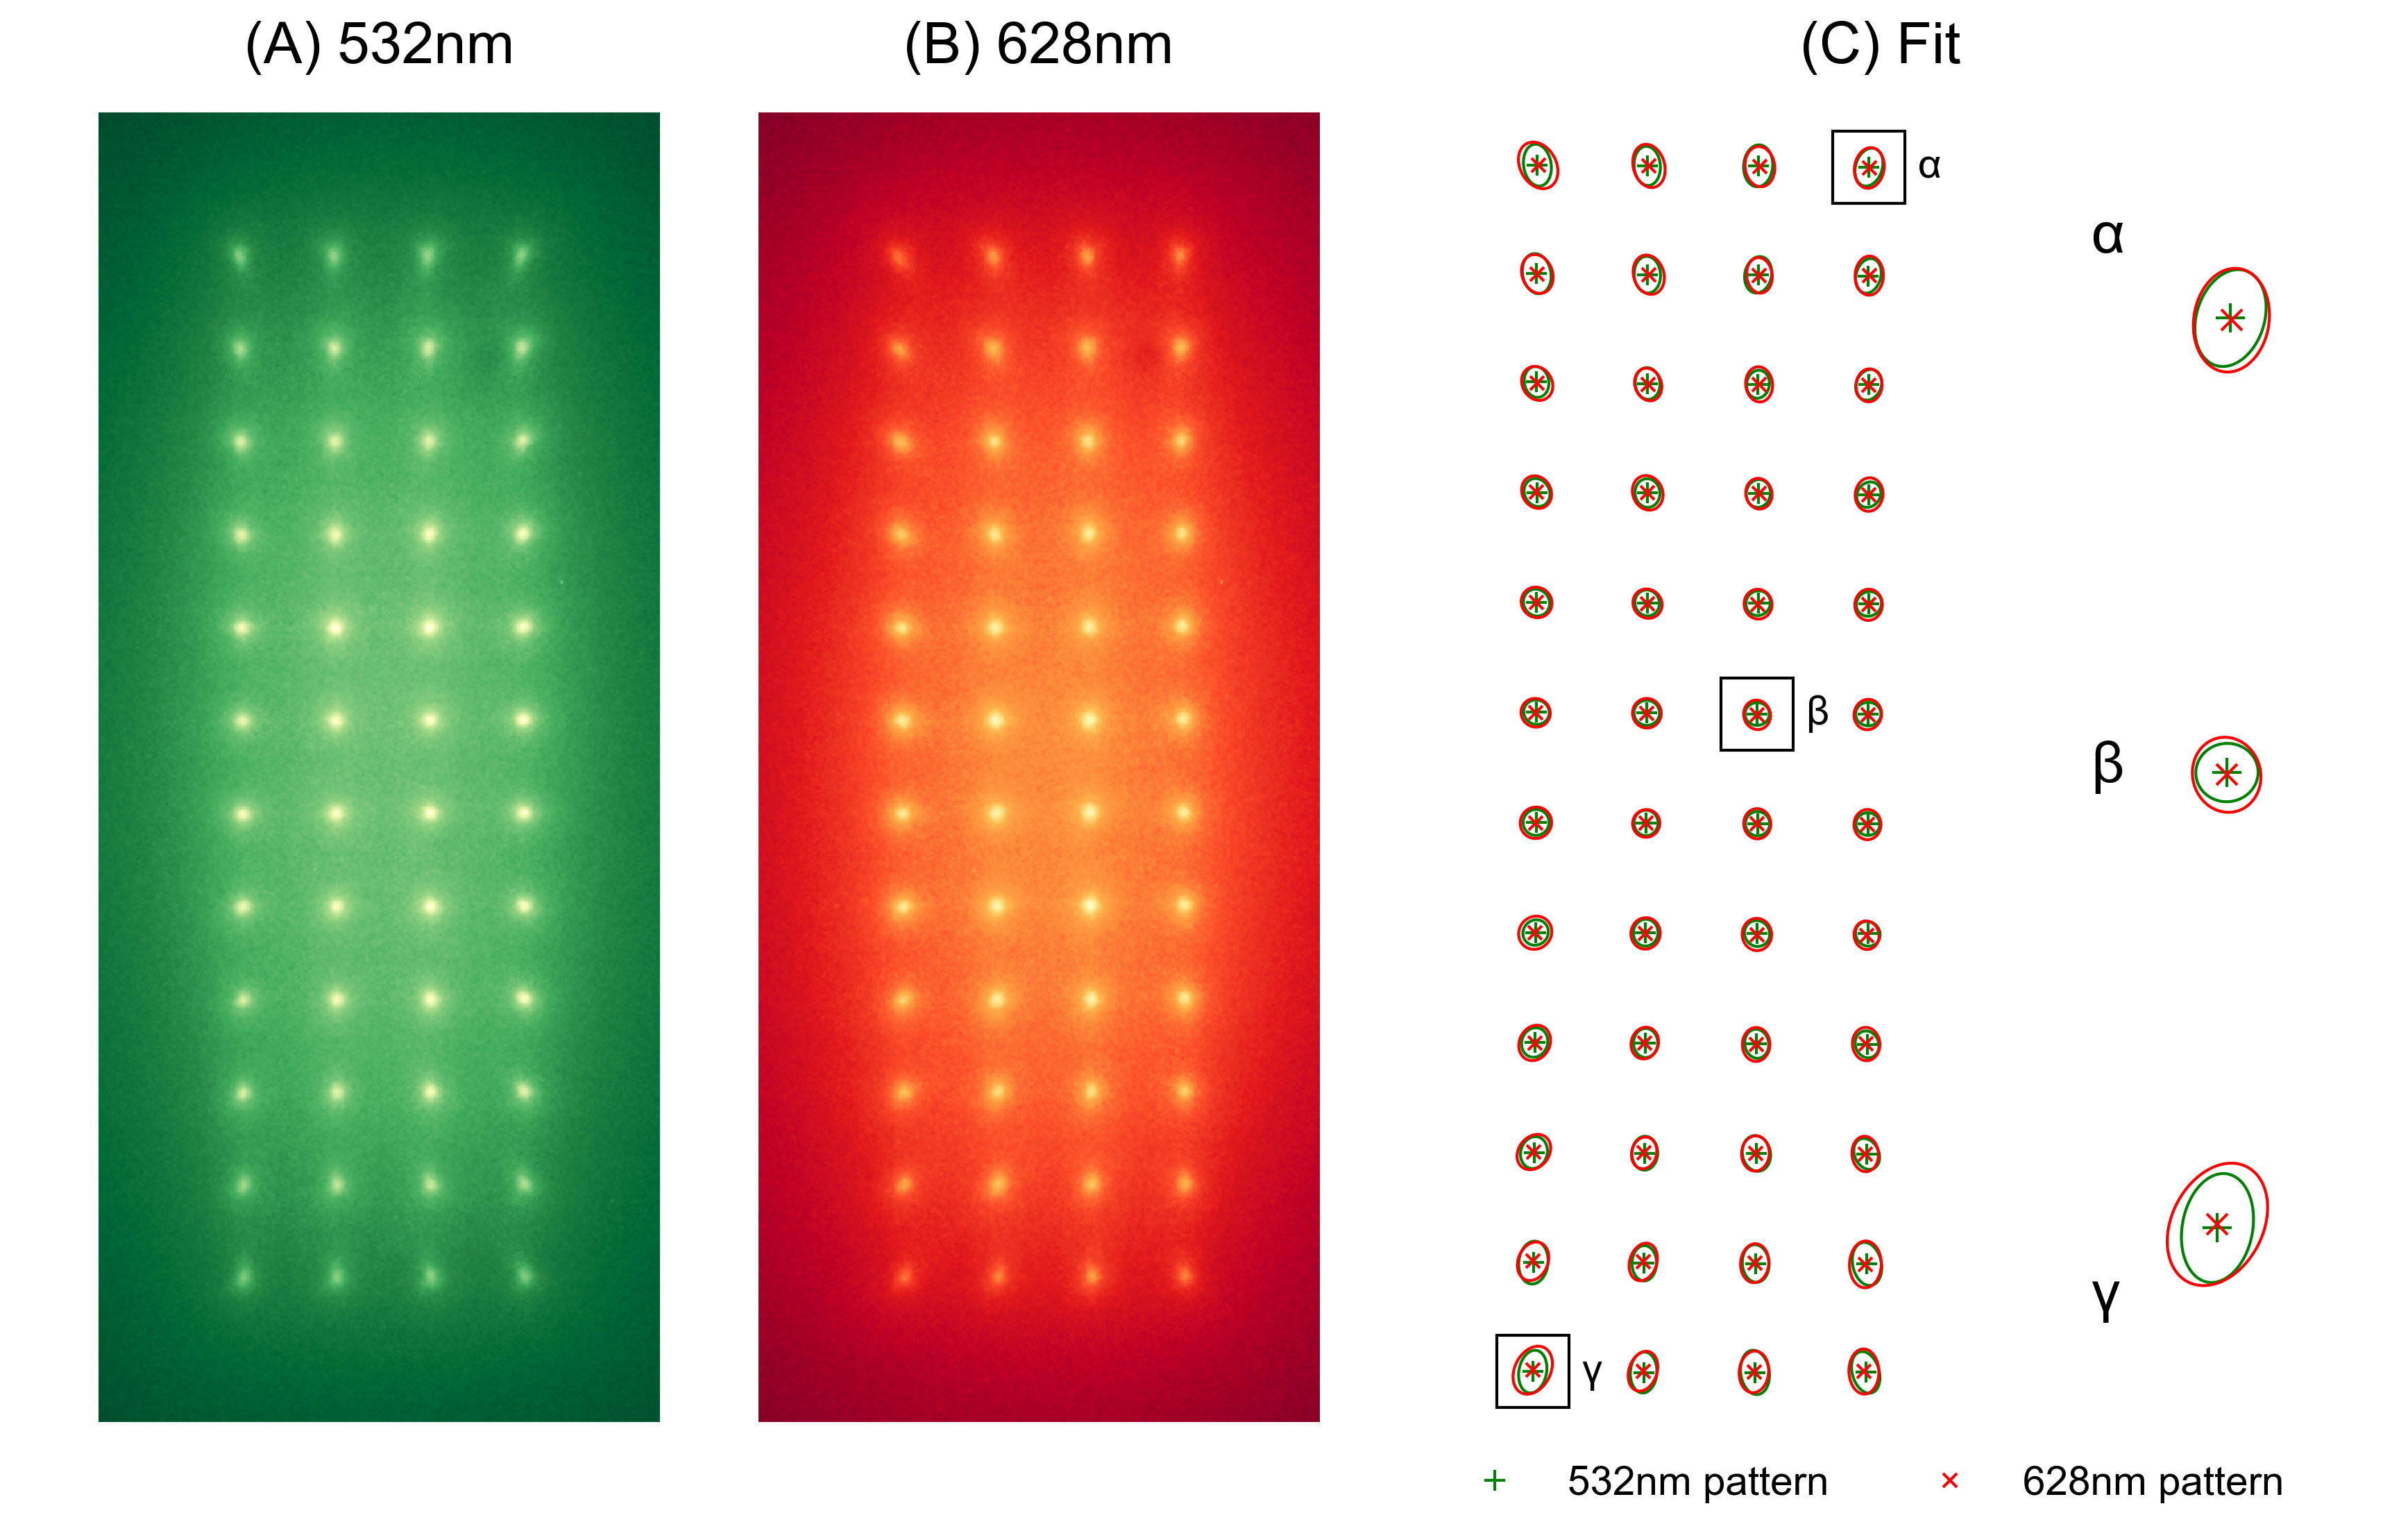
\includegraphics[width=\columnwidth]{figures/2017-04-28_conf9_G_conf14_R_green_red_pattern_and_fit}
    \caption{{\label{fig:patternfit}
    The 12x4 multispot pattern for green (A) and red (B)
    excitation and Gaussian fit of the spots (C). The pattern is acquired by
    a camera on the microscope side port (see Fig.~\ref{fig:setup}) using a
    solution of ATTO550 and ATTO647N dyes at high concentration ($\sim$100~nM).
    Fluorescent images obtained upon 532~nm or 628~nm laser excitation were
    acquired separately and are reported in green and red intensity levels
    in panels (A) and (B), respectively. Scale bars are 5~{\micron}.
    To assess the alignment,
    each spot in the two images is fitted with a 2D Gaussian function. Panel
    (C) reports an overlay of the fitted peak positions and a
    contour of the Gaussian waist for 532~nm (\emph{green}) and 628~nm
    (\emph{red}) images. A zoom-in for 3 representative spots is reported on
    the right. The elliptical shape and rotation of the Gaussian is
    due to geometrical aberrations.%
    }}
\end{figure}

\section{smFRET measurements}
\label{sec:smfret-meas}

\subsection{Analysis}
\label{sec:analysis}

Single-molecule measurements were performed with 40 base-pair (bp) dsDNA
samples labeled with dyes ATTO550 (D) and ATTO647N (A)
(ATTOTEC GmbH, Heidelberg, Germany)
attached to different DNA bases, yielding different inter-dye distances.

D-A separation of 12 and 22 base pairs (bp) were used in these experiments,
as they cover the typical range of distances that can be accurately measured
with smFRET using this dye pair.
Samples were diluted to single-molecule concentration ($\sim50$~pM) in TE50
buffer (10~mM Tris pH 8.0, 1 mM EDTA, and 50~mM NaCl).
Full details regarding these samples are provided in
ref.~\onlinecite{ingargiola_multispot_2017}.

We analyzed data using standard {\usalex} methods\cite{lee_accurate_2005}
with modifications required for smFRET-PAX\cite{doose_periodic_2007}.
The three steps of the analysis are:
(a) background estimation, (b) burst search, and (c) burst selection.
Background estimation, which is used to correct the burst counts
in the different photon streams, was performed in 10~s time windows
in order to account for possible variations during the measurement.
Burst searches were performed independently for each spot
using the sliding-window algorithm~\cite{fries_quantitative_1998}
and a constant-rate threshold for all spots~\cite{ingargiola_fretbursts:_2016}.

The main result of the {\usalex} analysis is a so-called E-S histogram,
a two-dimensional histogram where each burst is represented by a
pair of values $(E, S)$. $E$ is either the FRET efficiency or, more commonly
the uncorrected FRET efficiency, known as proximity ratio, $E_{PR}$.
$E_{PR}$ is easier to compute
and provides a suitable approximation for identifying sub-populations.
However, when the purpose is to extract D-A distances (which is not the
objective of this study), $E$ must be computed, requiring accurate
estimation of all the correction coefficients.
$S$ is the "stoichiometry ratio," a quantity ideally centered around 0.5 for
doubly-labeled species, 0 for A-only, and 1 for D-only species.
Note that D and A-only species also include
doubly-labeled molecules where one dye is fluorescently inactive
either in the blinking off state or bleached.
When using the simpler version without correction
(eq.~\ref{eq:S}), $S$ can depend on $E$ and, for doubly-labeled
molecules is only approximately centered around 0.5.
The use of the $(E, S)$ pair (corrected or uncorrected)
allows separation of singly and doubly-labeled species and
distinguishing FRET sub-populations in the doubly-labeled population.
Definition of all these quantities and a comparison with their ALEX
counterpart is reported in the appendix~\ref{sec:alex_pax}.

In this paper, we report proximity ratios $E_{PR}$ computed according to
eq.~\ref{eq:Epr}, and a ``modified stoichiometry ratio'' $S_u$ defined
in eq.~\ref{eq:Su}. $S_u$ is a variant of the classical
smFRET-PAX stoichiometry\cite{doose_periodic_2007}, which reduces the effect
of shot noise and improves the separability of D-only and FRET populations.
More details on $S_u$ can be found in appendix~\ref{sec:Su}.
Note that throughout this work the results of the two leftmost
spots in the second row are missing because of an active quenching circuit
(AQC) failure in the D-SPAD array.

\subsection{Peak photon rate}
\label{sec:peak-phrate}

\begin{figure*}
    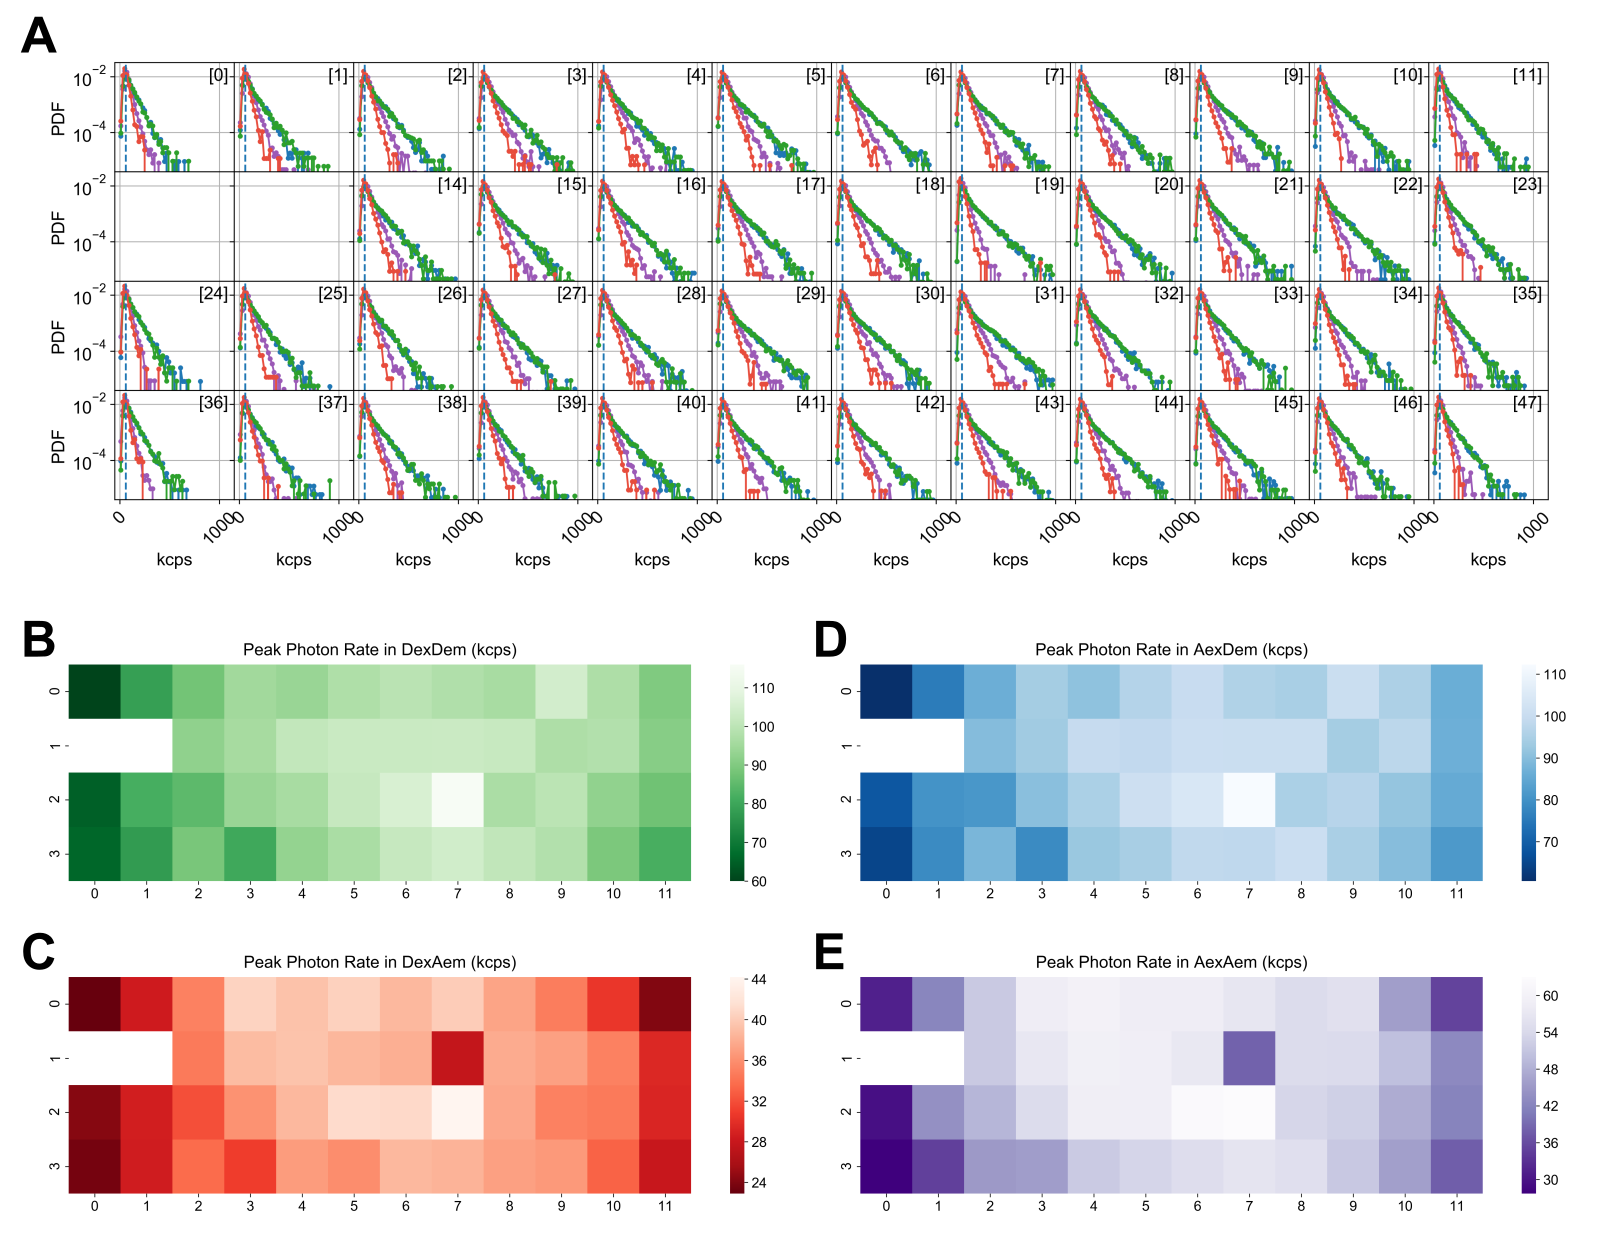
\includegraphics[width=\textwidth]{{figures/phrates_composite}}
    \caption{{\label{fig:phrates48_comp}
    Peak photon rates in each of the 48 spots for a dsDNA sample with
    D-A separation of 12bp.
    Panel A: full distribution of peak photon rates. Panels
    B-E: Mean of the peak photon rate distribution in different photon
    streams. Two lateral spots in the second row exhibit no signal because of
    two malfunctioning pixels in the D-SPAD array.
    Color-coding indicates different photon streams.
    Green $D_{ex}D_{em}$, red $D_{ex}A_{em}$, light blue $DA_{ex}D_{em}$,
    purple $DA_{ex}A_{em}$.%
    }}
\end{figure*}

\begin{figure}
    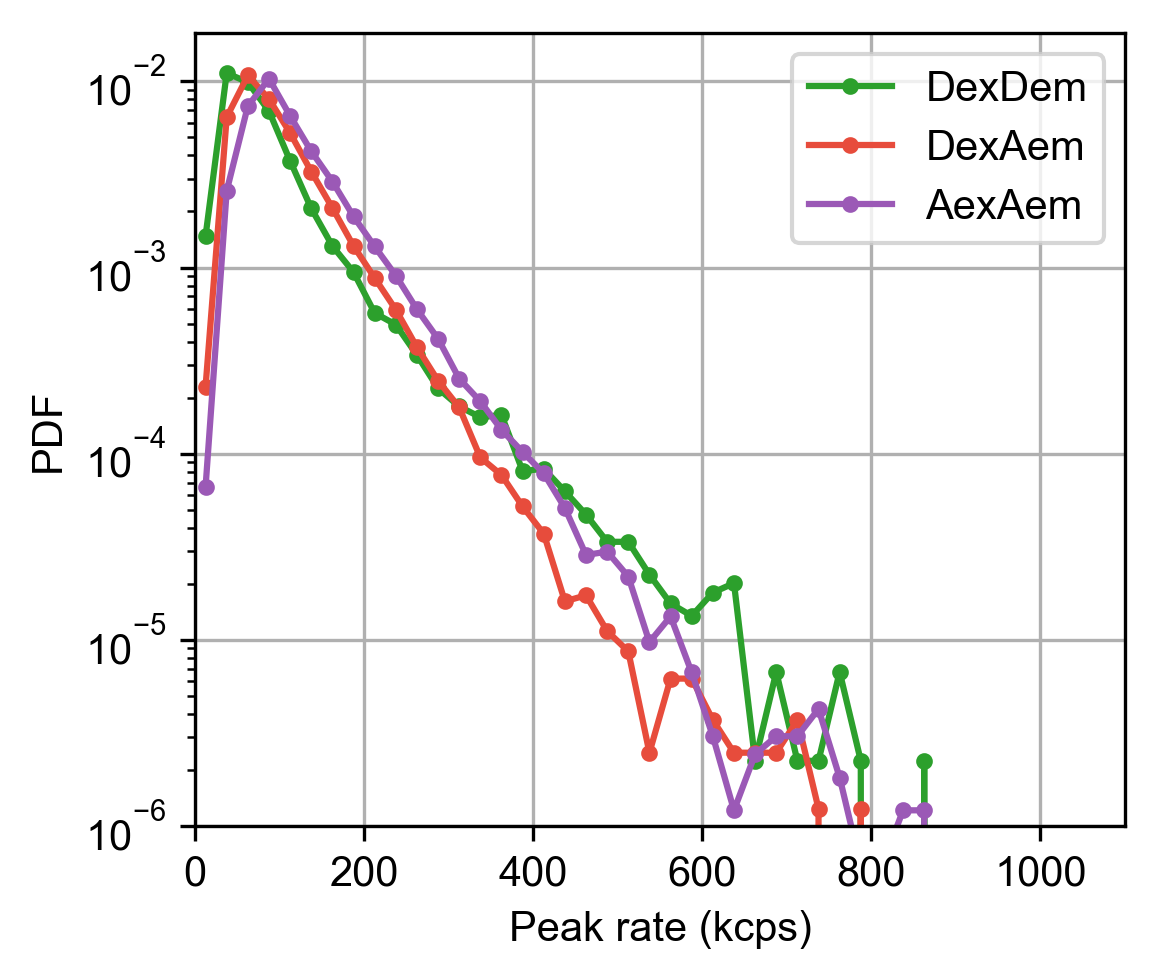
\includegraphics[width=0.8\columnwidth]{figures/2017-06-02_002_12d_usALEX_peak_phrate}
    \caption{{\label{fig:phrates_usalex}
    Distribution of peak photon rates in a single-spot {\usalex} measurement
    of the dsDNA sample with D-A separation of 12bp.
    Color-coding indicates different photon streams.
    Green $D_{ex}D_{em}$, red $D_{ex}A_{em}$,
    purple $A_{ex}A_{em}$.%
    }}
\end{figure}

We start by analyzing the peak photon rate reached in each burst,
a quantity that scales with peak PSF intensity\cite{ingargiola_multispot_2017}.
Fig.~\ref{fig:phrates48_comp} shows the background-corrected peak photon-rate
in each burst for the 48 spots. Panel A shows the full peak photon-rate
distributions with their characteristic exponential tails.
Panels B-E show heatmaps for different photon streams of the peak photon-rate
mean values i.e. the decay constant of the exponential tail.
Due to the Gaussian profile of the excitation beam and to geometrical
aberrations, the lateral pixels receive a lower signal intensity than central pixels.
As a result, the peak photon-rate decreases and fewer
single-molecule bursts are detected in the lateral spots.
While this effect decreases the overall maximum reachable throughput,
it does not influence the uniformity of the ratiometric quantities
$E_{PR}$ and $S$ across different spots.
Conversely, in Fig.~\ref{fig:phrates48_comp} (Panels C, E), we observe that the pixel
at position (1, 7) in the A-SPAD array systematically
detects fewer photons, an effect ascribed to a lower PDE of that pixel.
This effect causes a bias in $E_{PR}$ and $S$ quantities as shown below.

Fig.~\ref{fig:phrates_usalex} shows the distribution
of peak photon rates obtained with the {\usalex} setup.
Comparing Figs.~\ref{fig:phrates48_comp} Panel~A and~\ref{fig:phrates_usalex}
it is clear that reduced sensitivity in the A-SPAD array results in lower peak
photon rates in the $D_{ex}A_{em}$ (red) and $DA_{ex}A_{em}$ (purple) streams
in the 48-spot setup.

\subsection{E-S histograms}
\label{sec:EShist}

\begin{figure*}
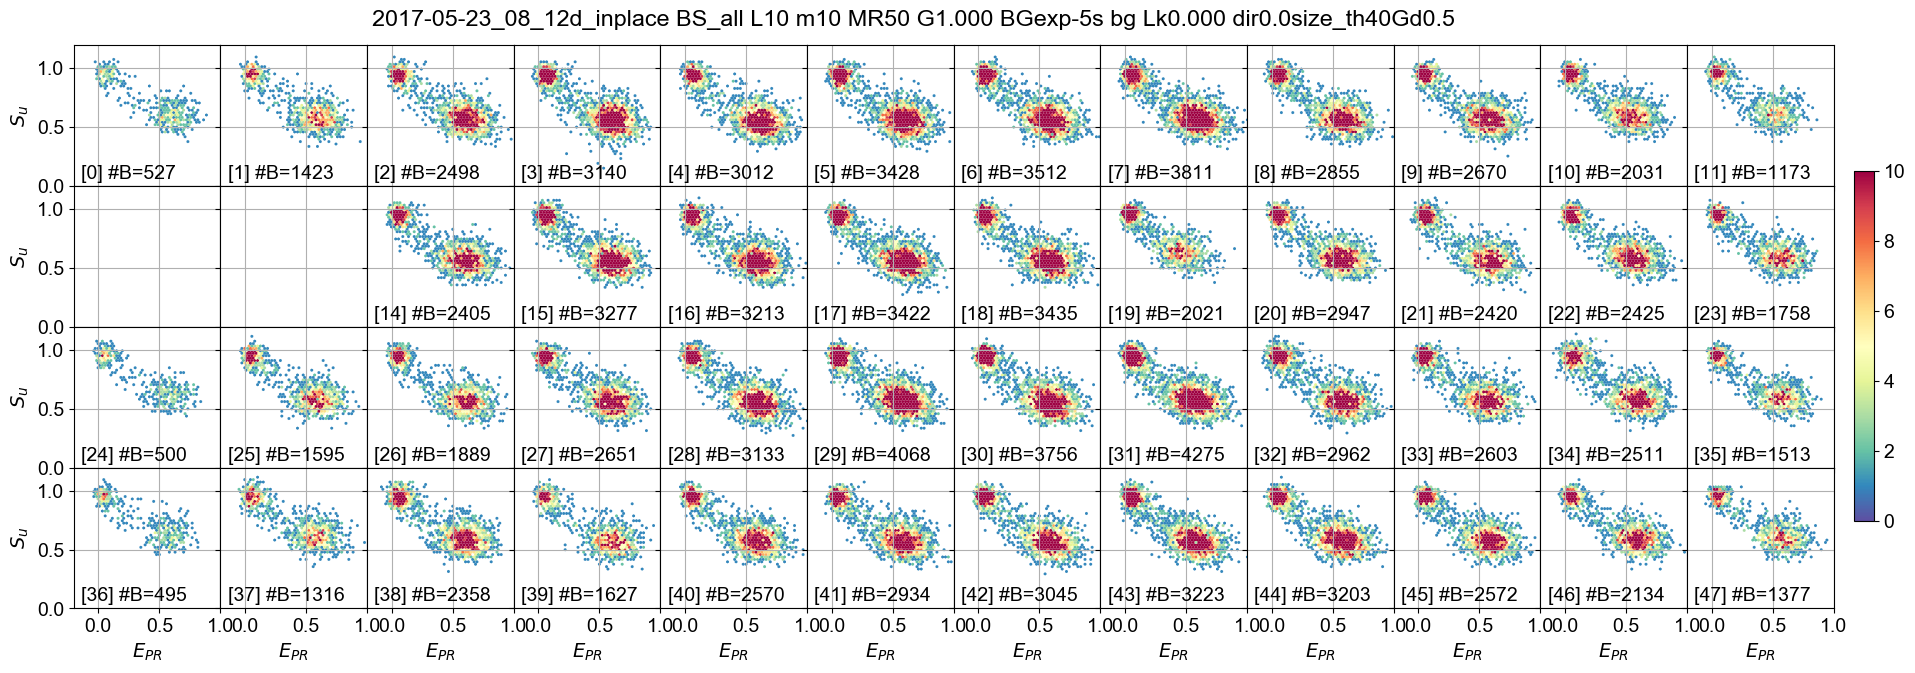
\includegraphics[width=\textwidth]{figures/2017-05-23_08_12d_48spot_alex_hist_Su_all-bursts}
\caption{{\label{fig:alexhist48all12d} $E_{PR}$ versus $S_u$
histograms for the different spots in the dsDNA sample with D-A separation of 12bp.
Two subpopulations are visible: D-only (around $E_{PR}=0$,
$S_u=1$) and FRET population (around $E_{PR}=0.6$,
$S_u=0.6$). Burst search was performed using all photons with
constant-threshold burst search (50~kcps). Burst selection was performed
on the total burst size after background correction, using a threshold of
40 photons. The legend in each subplot reports spot number
($[\cdot]$) and number of bursts (\#B).%
}}
\end{figure*}

\begin{figure*}
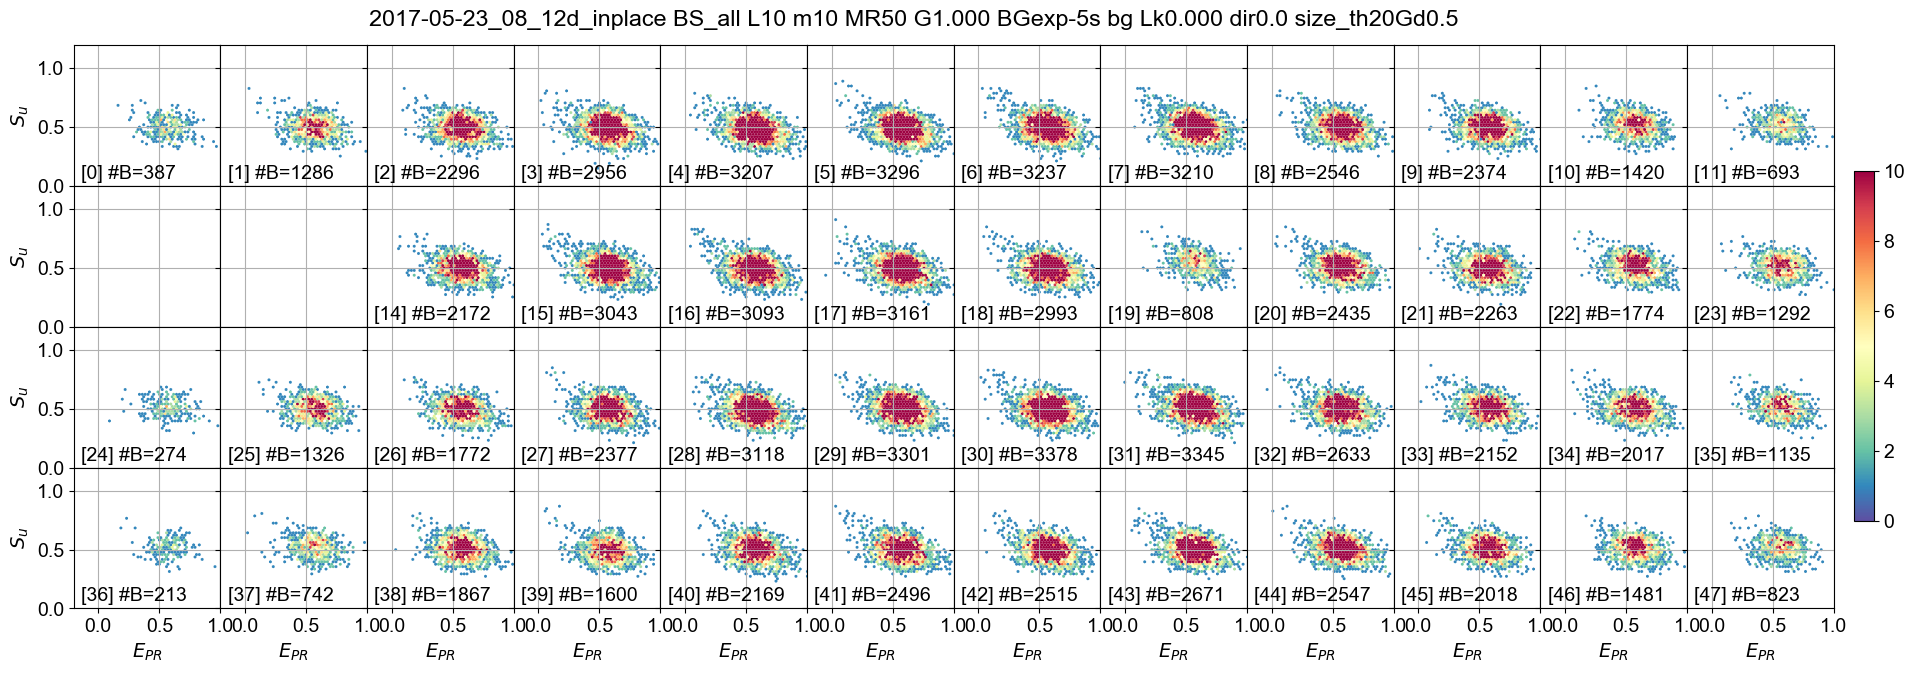
\includegraphics[width=\textwidth]{figures/2017-05-23_08_12d_48spot_alex_hist_Su_naa_AND_size_selection}
\caption{{\label{fig:alexhist48fret12d} $E_{PR}$ versus $S_u$
histograms for the different spots in the dsDNA sample with D-A separation of 12bp.
Data  analysis and
burst search are identical to figure~\ref{fig:alexhist48all12d}, while
burst selection was tailored to select only the FRET population: a burst is
selected if the number of counts in the $D_{ex}DA_{em}$ and $DA_{ex}A_{em}$
streams are both larger than 20. The legend in each subplot
reports spot number ($[\cdot]$) and number of bursts (\#B).%
}}
\end{figure*}

\begin{figure}
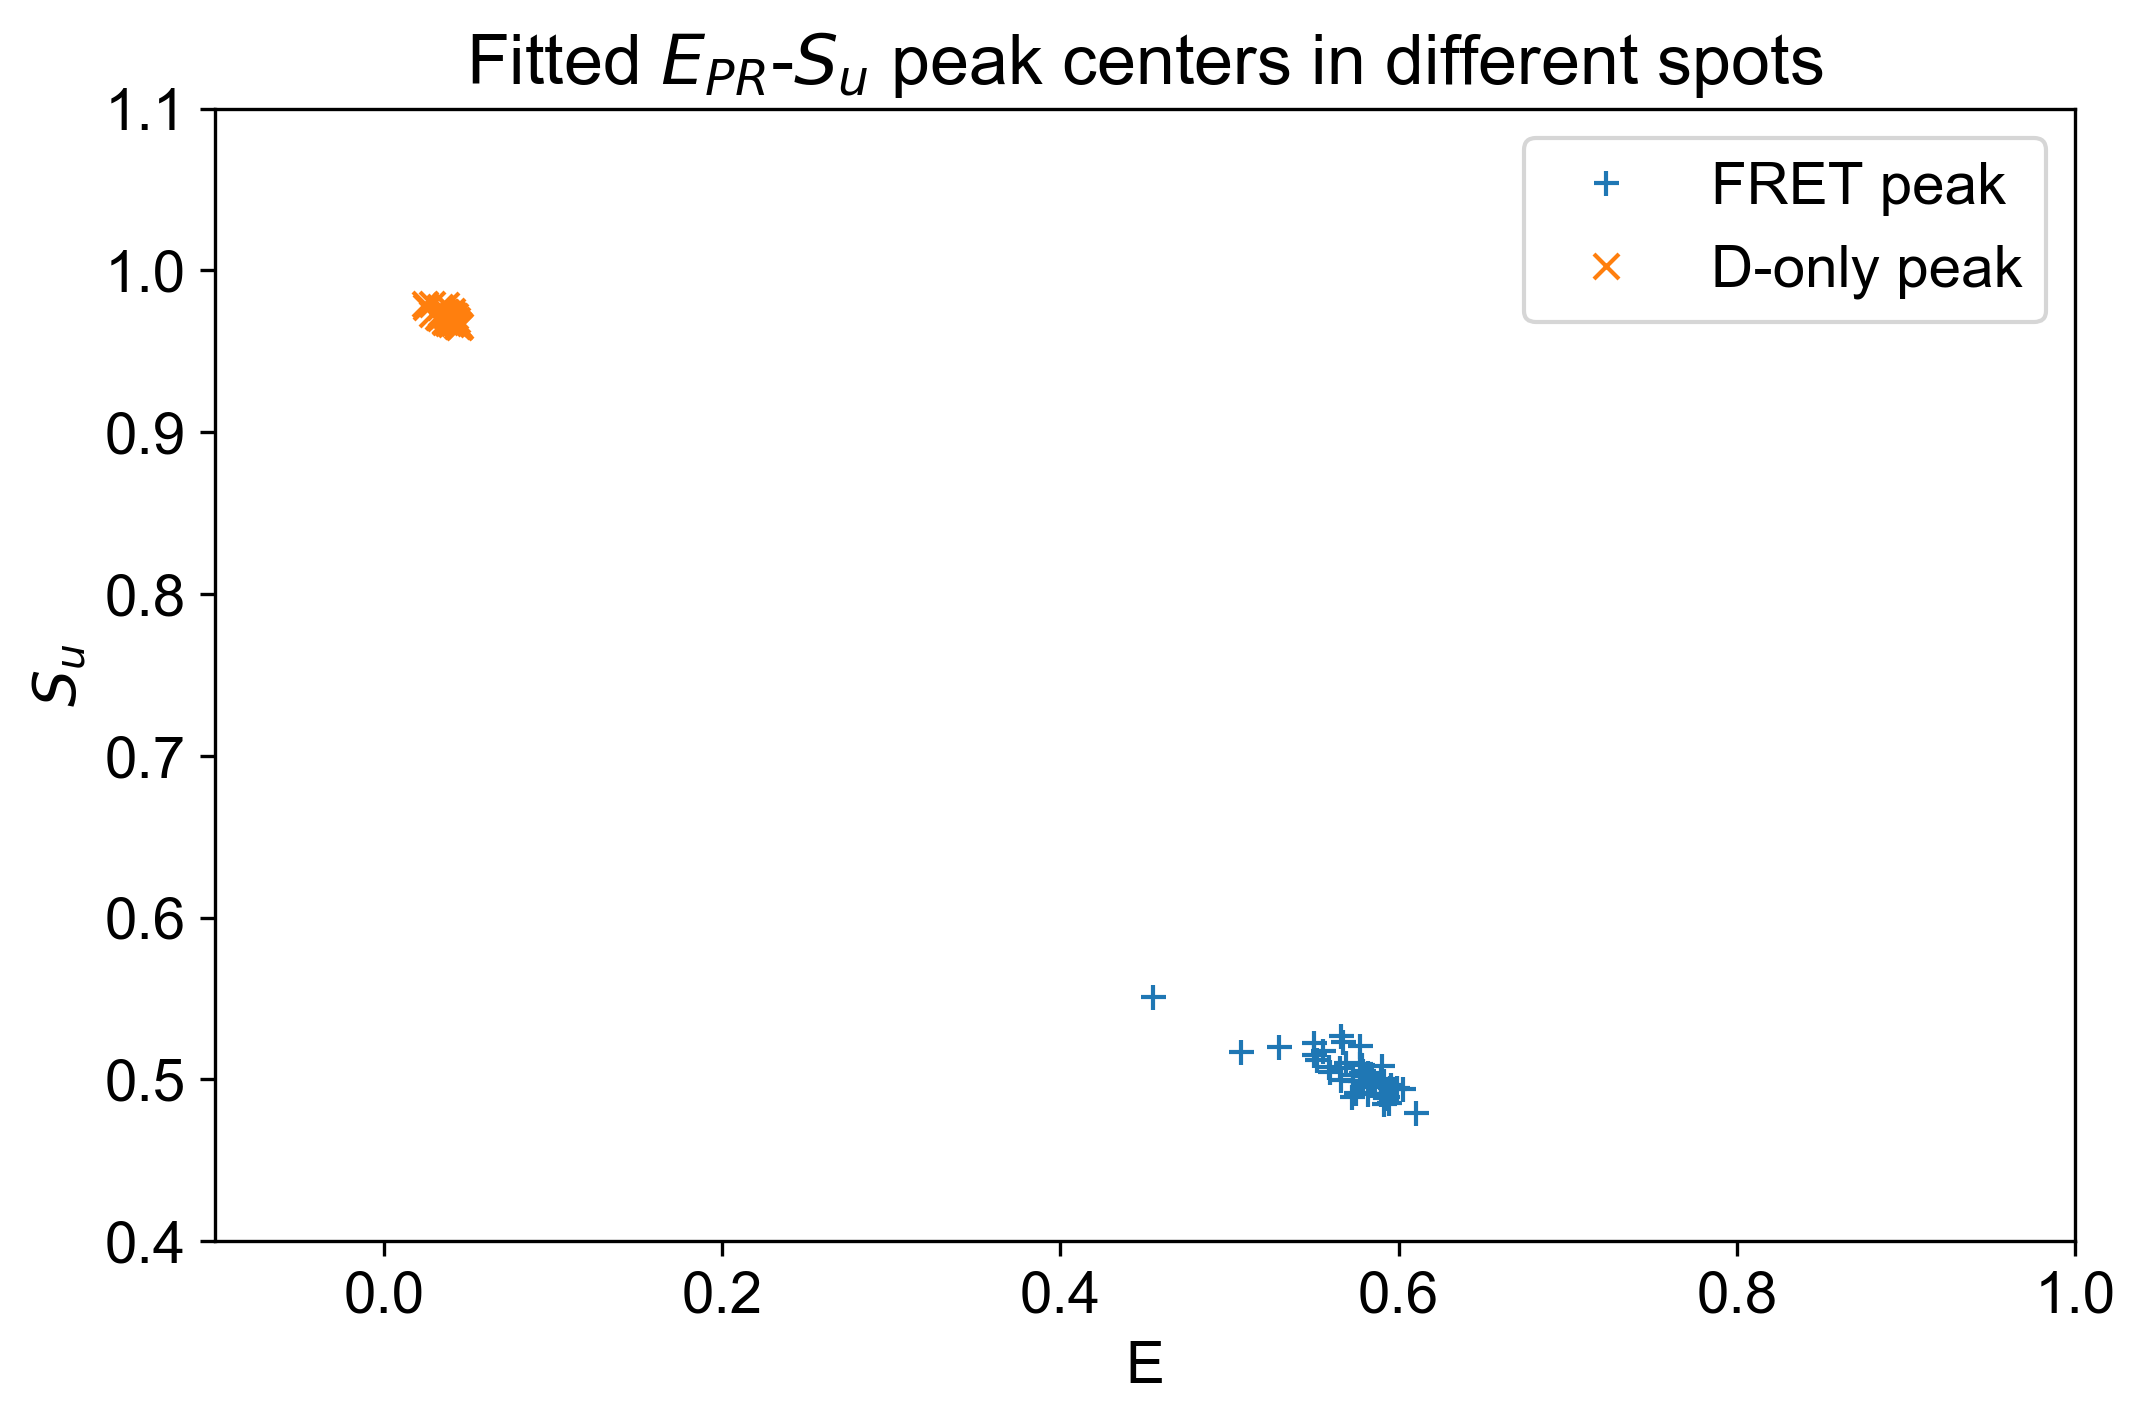
\includegraphics[width=0.8\columnwidth]{figures/2017-05-23_08_12d_FRET_vs_DO_fitted_Epr-Su_peak_position}
\caption{\label{fig:fittedFRETscatter}
Scatter plot of the fitted $E_{PR}$, $S_u$ peak
position in the different spots for the D-only (\emph{orange cross})
and FRET populations (\emph{blue plus}). Values were obtained by simple Gaussian
fitting of the 1-D histogram of $E_{PR}$ and $S_u$ after a bursts selection
that isolated D-only and FRET populations, respectively.}
\end{figure}

\begin{figure*}
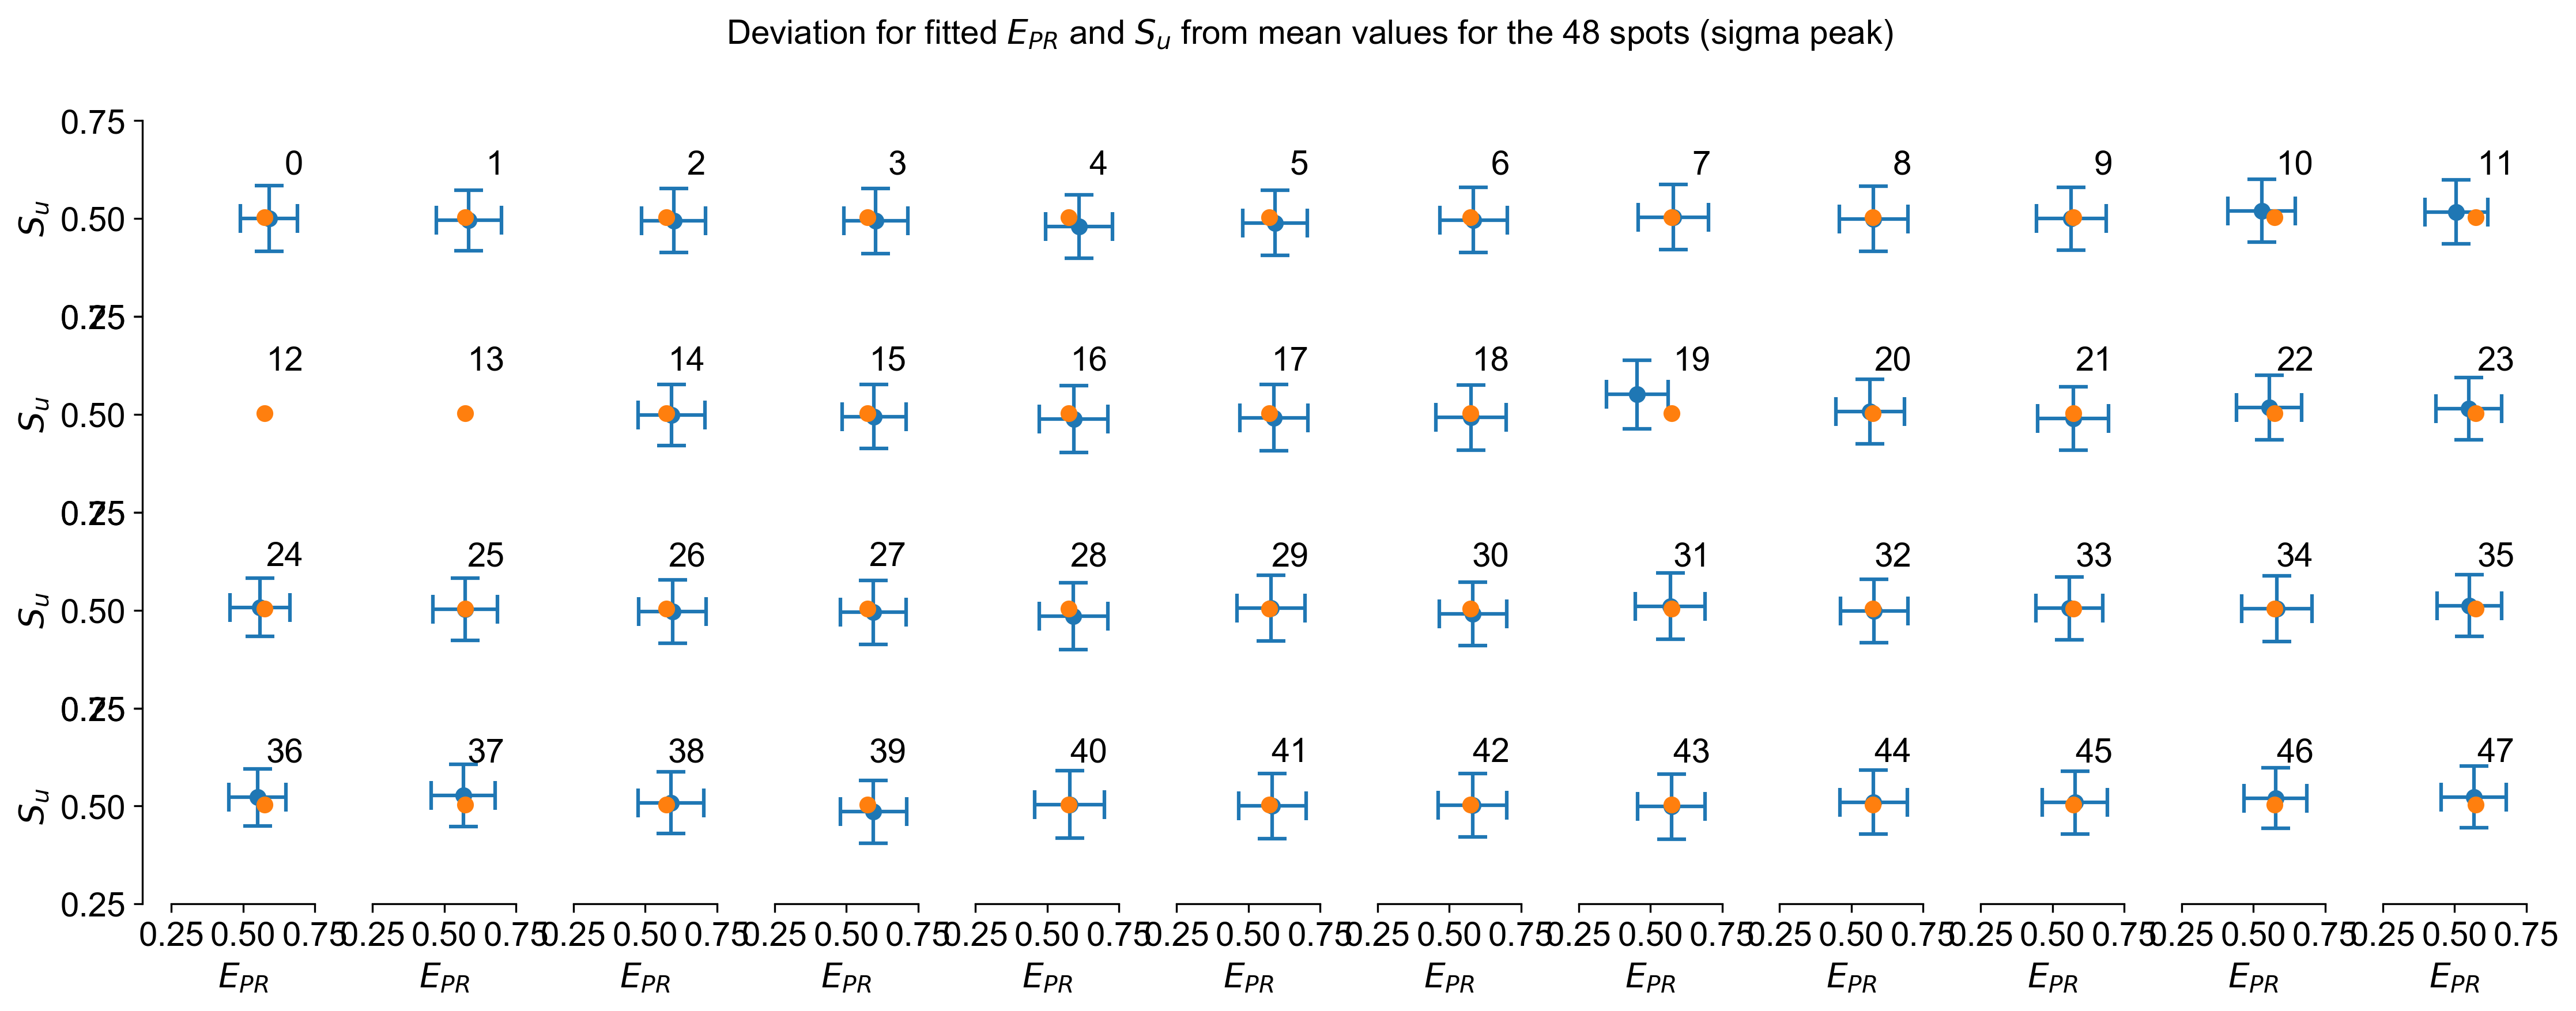
\includegraphics[width=\textwidth]{figures/2017-05-23_08_12d_48-spot_Epr-Su_peak_position_deviation_from_mean}
\caption{{\label{fig:fretfit48vsmean} Fitted FRET peak position ($E_{PR}, S_u$,
\emph{blue dots}) and $\pm 1 \sigma $ of the fitted Gaussian
(\emph{blue error bars}) for the 48 spots. As a reference, the mean
$E_{PR}, S_u$ across the 48 spots (\emph{orange dot}) is reported
in each subplot.  The spot number is indicated in the top right corner of
each subplot.%
}}
\end{figure*}


After the initial burst search, it is necessary to apply a burst selection
criterion to reject the smallest burst which dominates the distribution.
Fig.~\ref{fig:alexhist48all12d} shows the E-S histogram for the
dsDNA sample with D-A separation of 12bp,
after selecting bursts with photon counts from all the streams
larger than the threshold.
We observe that D-only and FRET populations (respectively top left corner
and center in the 2-D histogram) are clearly distinguishable in most channels.
Moreover, as shown in Fig~\ref{fig:alexhist48fret12d}, it is easy to isolate
the FRET population(s) by applying a burst
selection on the $DA_{ex}A_{em}$ counts and on $D_ex$ counts.
The separation of FRET from singly-labeled species is the primary advantage
of dual laser excitation.

Without any further calibration, the spread across different channels
is limited and does not affect the ability to distinguish subpopulations.
This is evident in Fig.~\ref{fig:fittedFRETscatter} which shows the
$E_PR$ and $S_u$ peak center position in different spots for
both D-only and FRET populations.
Fig.~\ref{fig:fretfit48vsmean} shows the center and $\pm1\,\sigma$
range of fitted E-S peaks for the FRET population (blue dot and error-bar)
for each channel.
The orange dot is the mean center peak position of the FRET population
across all the spots. We note that, for almost all channels, the
deviation of the peak position is very well below the $\pm1\,\sigma$
range, with exception of channel 19, where lower PDE of the A pixel
causes a larger deviation from the peak position.
In Fig.~\ref{fig:fittedFRETscatter} and~\ref{fig:fretfit48vsmean}
we present results without channel calibration for the purpose
of illustrating the raw performance of the system.
It is possible, however, to reduce the channel-to-channel variations
on E-S peak position by applying a per-spot calibration briefly
described in the next section (with full details in
appendix~\ref{sec:perchcorr}). For comparison,
the E-S histogram for a low-FRET dsDNA (D-A separation 22bp) is reported
in appendix~\ref{sec:moredata}, Fig.~\ref{fig:alexhist48all22d}.


\subsection{Pooling data from all channels}
\label{sec:alexpax-comp}
To illustrate the high-throughput performance of the 48-spot system, we
build an ALEX histogram accumulating bursts from all spots for a short
time window of 15~s (Fig.~\ref{fig:alex_mspot_15}). In principle,
non-uniformities between different channels can be taken into account
by decomposing $\gamma$ and $\beta$ in two factors: one that is an average
value for all the spots and another that is a per-spot "relative" adjustment.
The per-spot component of $\gamma$ and $\beta$ can be easily computed
from a measurement of a static FRET sample
(details in appendix~\ref{sec:perchcorr}).
Fig.~\ref{fig:alex_mspot_15}, for simplicity and because of the good uniformity
across spots, we report raw $E_{PR}$ and $S_u$ values without
any spot-specific adjustments.

For comparison, Fig.~\ref{fig:alex_sspot_15} shows a similar histogram obtained
by accumulating bursts for 15~s during a measurement of the same sample using the
single-spot {\usalex} setup. While we observe that
the total number of bursts  detected in the multispot measurement
is about 12 times larger than in the single spot measurement, a quantitative
comparison cannot be done because the measurements were taken on different
dilutions in the two setups. Apart from the difficulty in controlling
the sample concentration with high accuracy, there are other reasons why the
burst number would not exactly scale with the number of spots.
First, in the multispot setup, it is difficult to estimate the power
in each spot because the intensity is not uniform and lateral spots
receive less power. The power is calibrated such that, in the central spots,
we obtain a signal in the D-channel comparable to the single-spot measurements
(which used 180~\textgreek{μ}W @ 532~nm). The lateral spots receive less
power and therefore detect a lower number of bursts.
Second, the detection efficiency of the SPAD array in the red region
of the electromagnetic spectrum is lower than that of the corresponding
SPAD in the single-spot setup (see section~\ref{sec:detectors}),
reducing total burst size and therefore the number of bursts selected with
a given threshold.


\begin{figure}
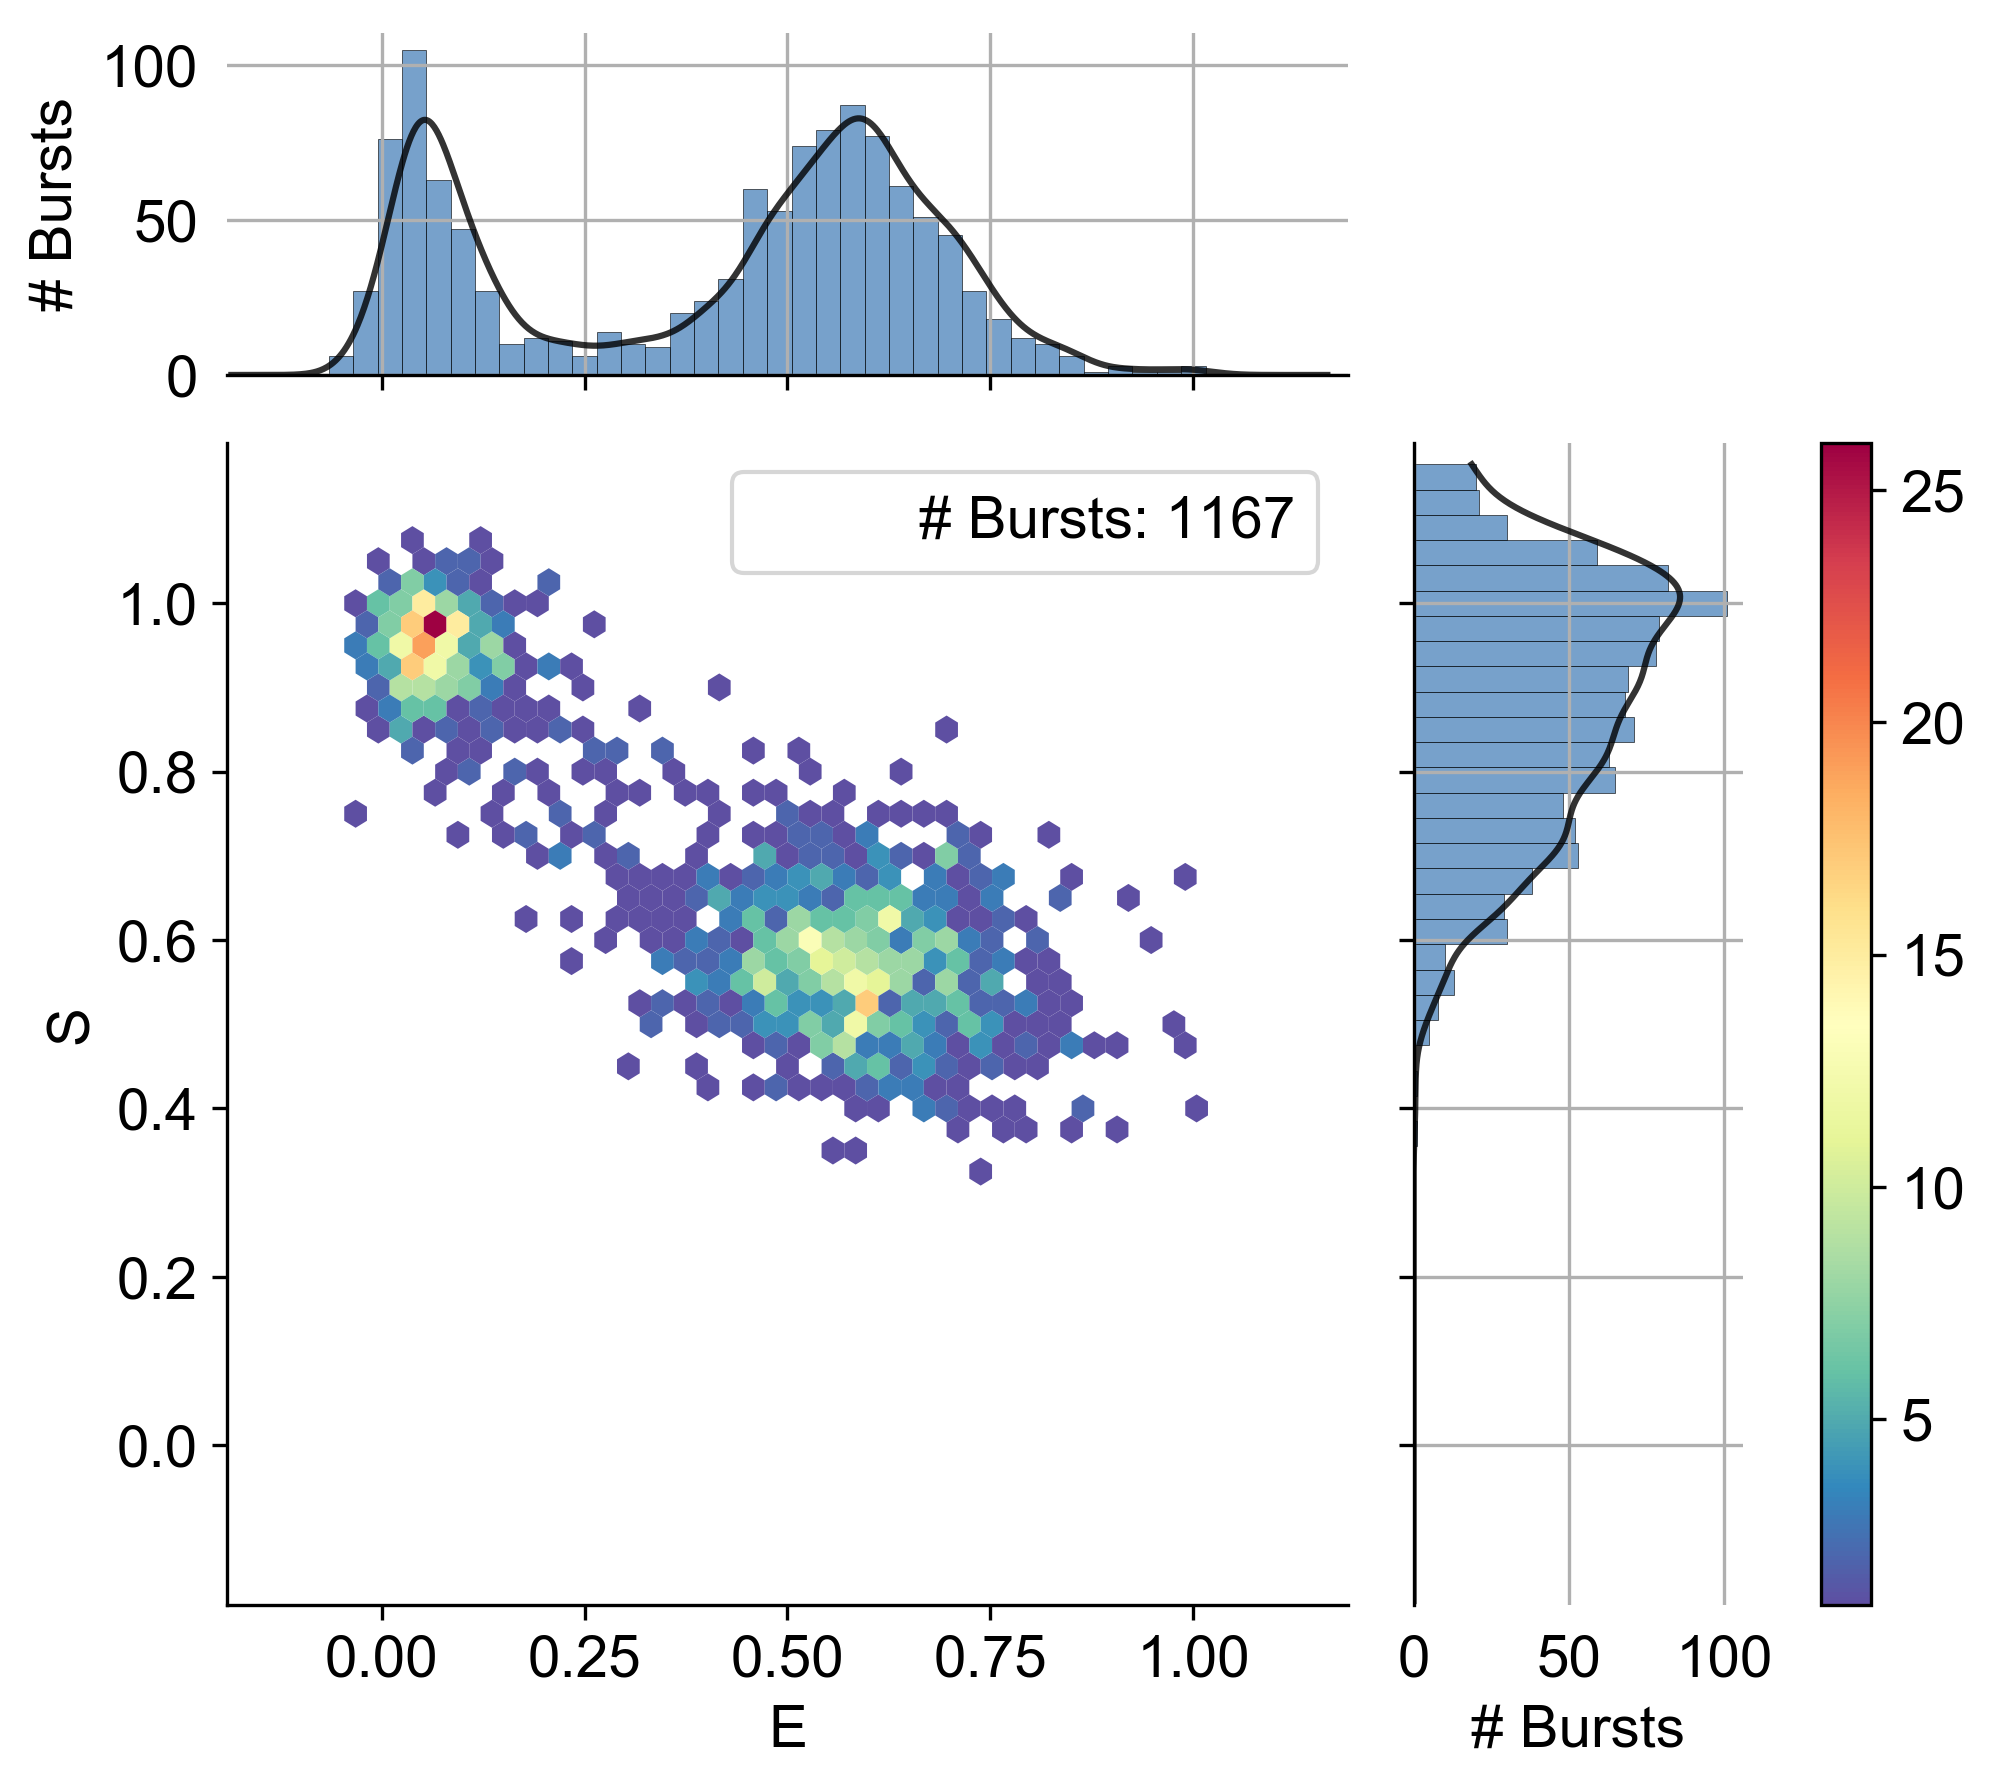
\includegraphics[width=\columnwidth]{figures/2017-05-23_08_12d_alex_jointplot_15s}
\caption{\label{fig:alex_mspot_15}
Multispot ALEX histogram obtained from 15~s of acquisition by pooling bursts
from all 48 spots.}
\end{figure}

\begin{figure}
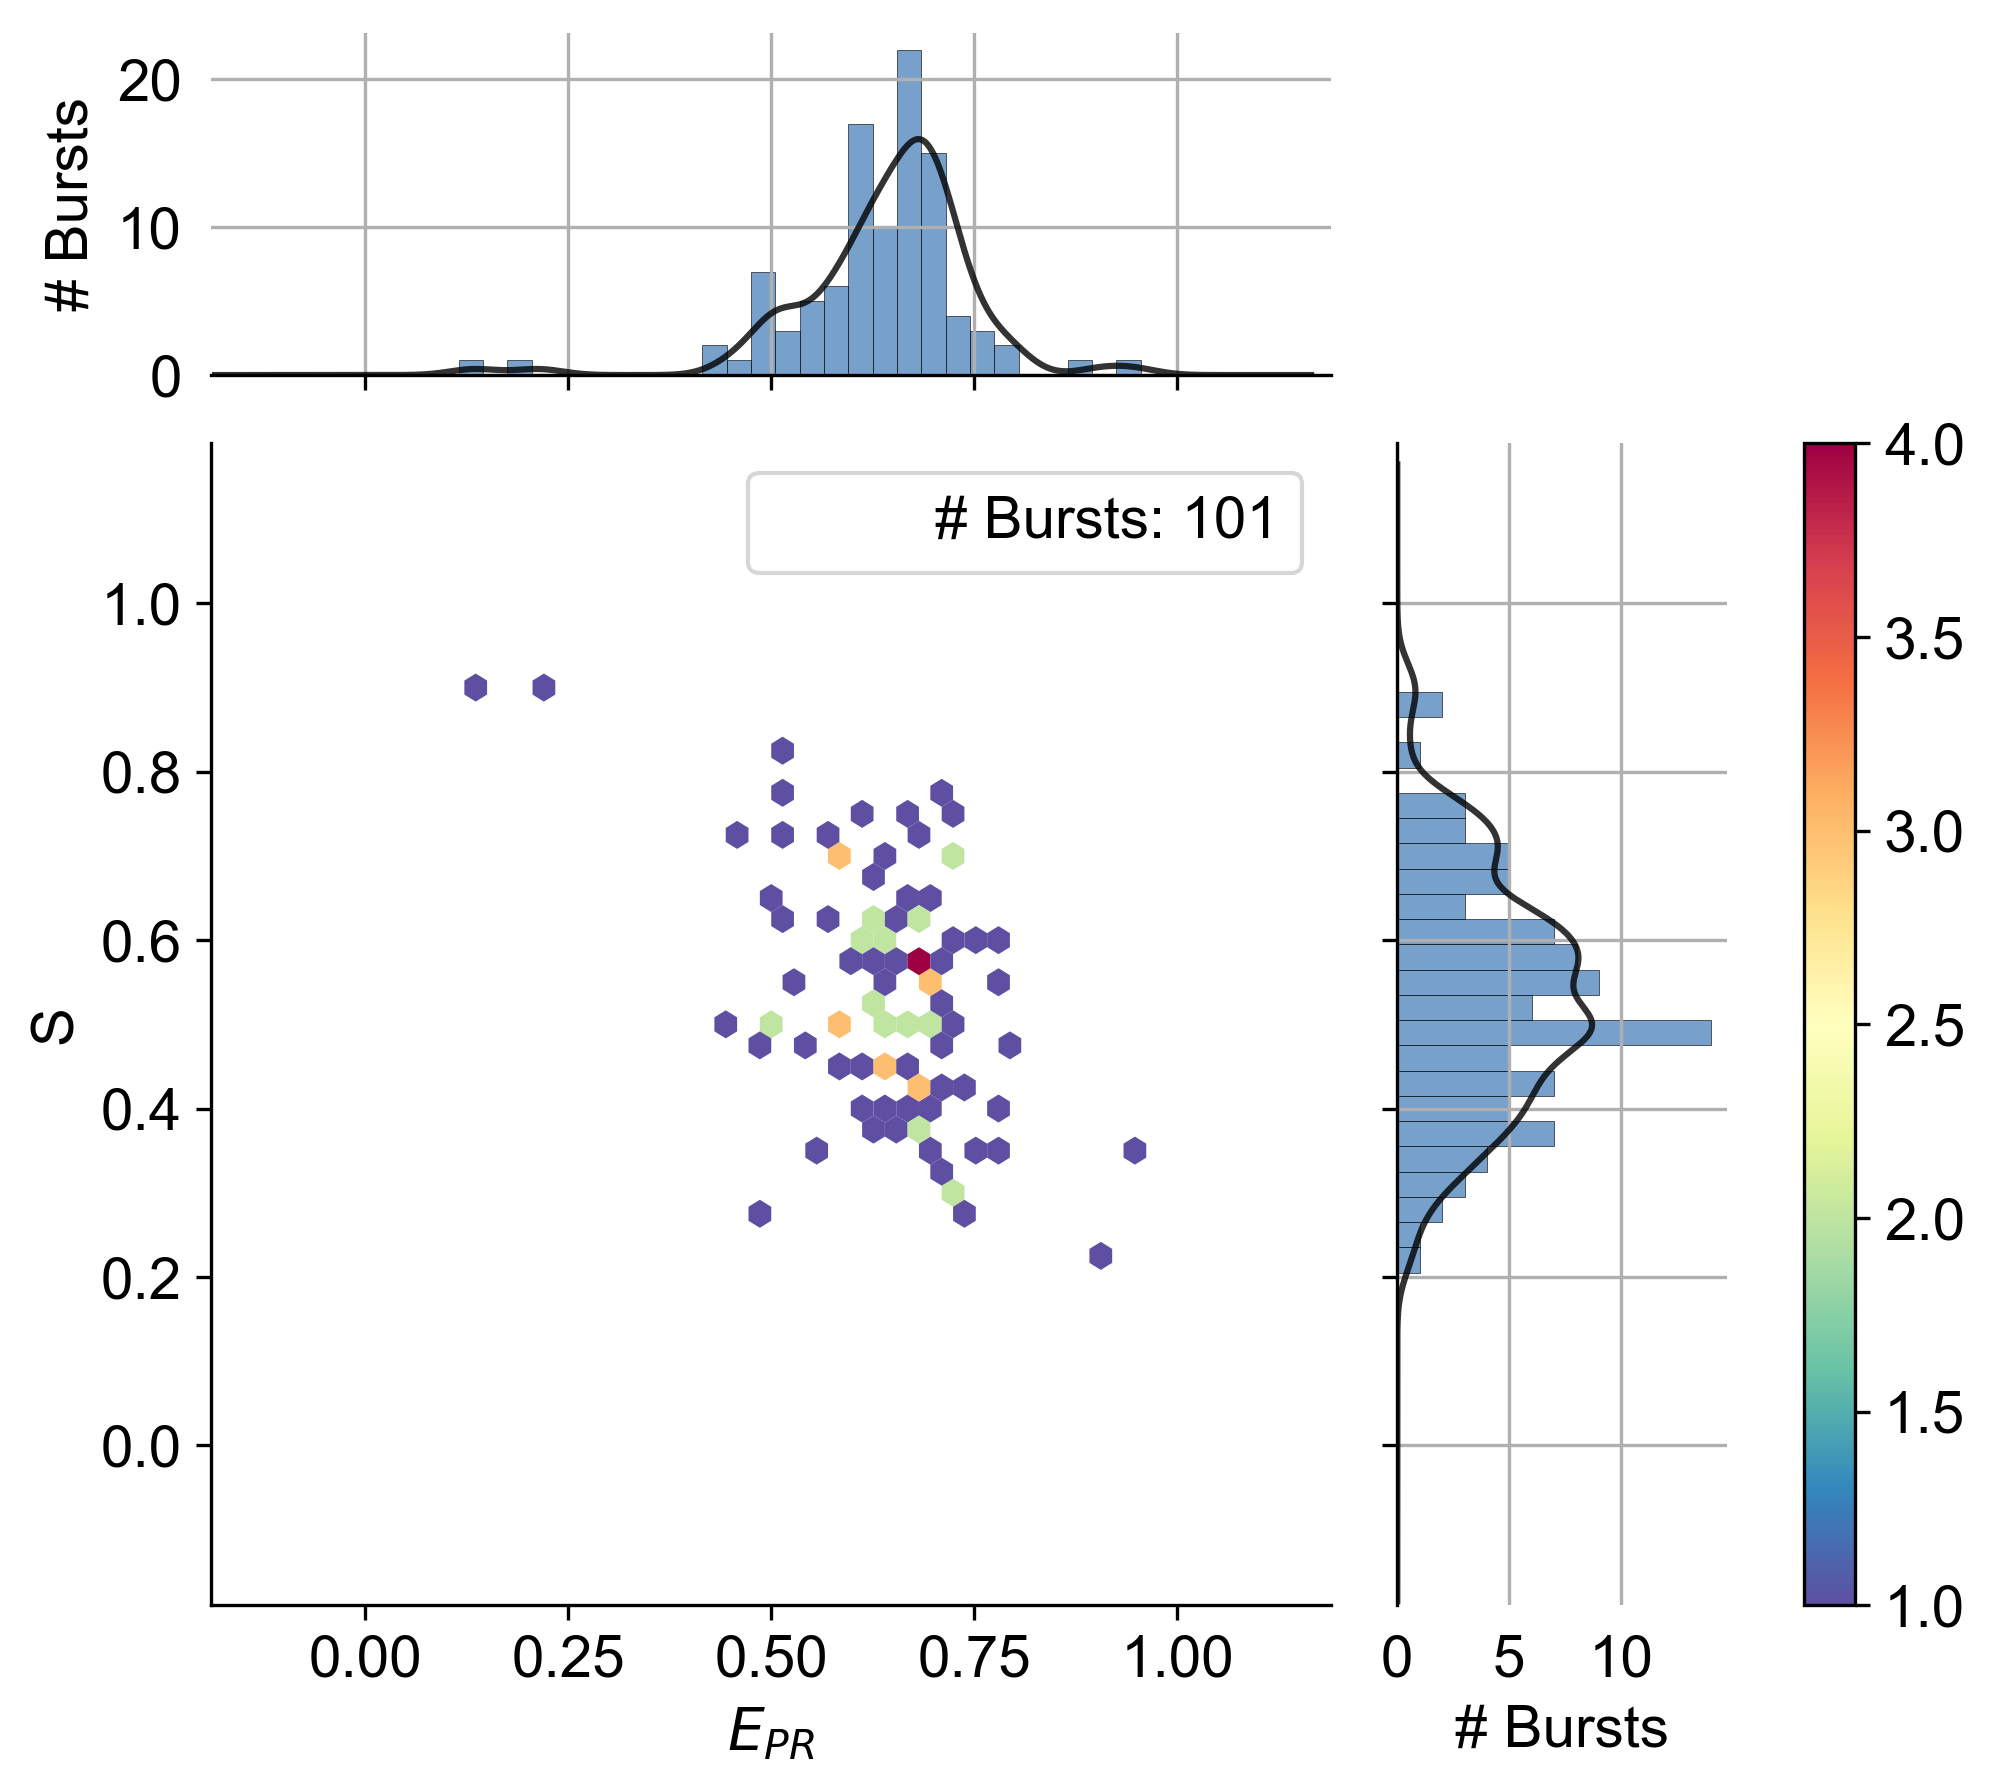
\includegraphics[width=\columnwidth]{figures/2017-06-11_000_12d_alex_jointplot_15s}
\caption{\label{fig:alex_sspot_15}
Single-spot ALEX histogram obtained from 15~s of acquisition for the same
sample as in Fig.~\ref{fig:alex_mspot_15}.}
\end{figure}

\section{Conclusion}

We have described a new 48-spot single-molecule FRET setup
designed for high-throughput single-molecule assays.
Compared to our previous multispot setup~\cite{ingargiola_multispot_2017},
the number of spots was increased six-fold with a corresponding increase
in throughput.
While larger SPAD arrays have been demonstrated,
they are fabricated using standard high-voltage CMOS processes
resulting in poorer photon-counting performance than the custom technology
process employed here. Convincing applications in cell FCS and FLIM,
among others, have been published with these CMOS SPAD
arrays~\cite{colyer_ultra_2011,burri_65k_2014,buchholz_fpga_2012,kloster-landsberg_note:_2013,kufcsak_time-resolved_2017,kufcsak_time-resolved_2017},
(for a comprehensive review see~\onlinecite{bruschini_ten_2017})
but they remain a long way off from offering the sensitivity needed for
single-molecule applications.

Compared to our previous works~\cite{ingargiola_multispot_2017,ingargiola_16ch_2017},
a second alternating excitation laser was incorporated,
and the corresponding alignment hurdles were solved,
permitting sorting of single-molecules according to their
D-A stoichiometry. In particular, we have shown that the setup
allows identifying singly and doubly-labeled species over the full range
of FRET efficiencies, opening the door to a much wider range of assays
than was previously possible.

We presented a detailed description of the multispot setup and alignment
procedure, which incorporates a number of technical solutions of potential
interest for other applications.
We also illustrated the smFRET measurement capabilities of the new setup
using doubly-labeled dsDNA molecules as a proof of principle
demonstration for sub-population separations and high-throughput measurements.
Finally, we provided a comparison of its performance with that
of a standard single-spot (confocal) {\usalex} setup.
Applications of this new instrument to the study of the initial
stages of bacterial transcription and high-throughput diagnostics
will be explored in future work.

\begin{acknowledgments}
The authors thank Luca Miari for help in the initial stage of this project,
Mr. Yazan Alhadid and Dr. Eitan Lerner for help with single-molecule
sample preparation and Dr. Eitan Lerner for critical reading of the manuscript.
We thank Dr. Bentolila for the generous loan of a LCOS SLM from the
Advanced Light Microscopy/Spectroscopy Shared Resource Facility at
the California NanoSystems Institute at UCLA.
Research reported in this publication was supported by the National Institute
Of General Medical Sciences of the National Institutes of Health under
Award Number R01GM095904 \& R01 GM069709, and by the National Science
Foundation under Award Number MCB 1244175.
The content is solely the responsibility of the authors and does not
necessarily represent the official views of the National Institutes of
Health or the National Science Foundation.
Conflict of interest statements: S. Weiss discloses intellectual
property used in the research reported here.
The work at UCLA was conducted in Dr. Weiss's Laboratory.
M. Ghioni discloses equity in Micro Photon Devices S.r.l. (MPD).
No resources or personnel from MPD were involved in this work.
\end{acknowledgments}


\appendix

\section{Detailed setup description}
\label{sec:setup}

The setup (Fig.~\ref{fig:setup}) comprises two excitation CW lasers at
532~nm and 628~nm (2RU-VFL-Series, MPB Communications Inc., QC, Canada).
For each laser, a half-wave plate and polarizing beam splitter are used
for polarization and intensity control, as the polarization orientation
must be aligned along the direction required by the LCOS-SLM. The
628 nm laser is directed through an acousto-optical modulator (P/N 48058
PCAOM, electronics: P/N 64048-80-.1-4CH-5M, Neos Technology, Melbourne,
FL, USA) used for {\microsec} time-scale modulation, and the 532~nm
laser is not modulated.
Each laser goes through a first beam expander (Keplerian
telescope, doublet lenses: 50~mm and 250~mm focal lengths). Two periscopes
bring the beams to a raised optical breadboard where a microscope body
(X71, Olympus Corporation, Japan) is fixed with its bottom port sitting
over a circular aperture. Beyond the periscope, each beam goes through a
second adjustable beam expander (3X, P/N 59-131, Edmund Optics Inc.).
The red laser is reflected off mirrors $M1_R$ and
$M2_R$ and phase-modulated by the ``red'' LCOS-SLM (P/N
X10468-07, Hamamatzu, Japan), before passing through the dichroic mirror
$D_{MIX}$. The green laser is reflected off $M3$,
phase-modulated by the ``green'' LCOS-SLM (P/N X10468-01, Hamamatzu),
and combines with the red excitation via the dichroic mirror
$D_{MIX}$ (T550LPXR, Chroma Technology Corp, VT, USA). Both
beams are recollimated by the $L_3$ lens (f=250~mm,
AC508-250-A, Thorlabs) and focused into the sample by a high-NA
objective lens (UAPOPlan 60x, NA 1.2, Olympus) after being reflected off
the excitation dichroic mirror $DM_{EX}$ (Brightline
FF545/650-Di01, Semrock Inc., NY, USA). The excitation pattern forms a
dual-color 12x4 array of spots into the sample matching the geometry of
the two SPAD arrays. The fluorescence emission is collected by the same
objective lens, passes through the excitation dichroic
$DM_{EX}$ and is focused by the microscope tube lens $L_2$ either on
the side or the bottom port of the microscope. The side port mounts a
sCMOS camera (Grasshopper3 GS3-U3-23S6M-C, FLIR Integrated Imaging
Solutions Inc., BC, Canada) used during alignment while the bottom port
redirects the beams toward the emission path. Here, a relay lens
$L4$ (f=100~mm, AC254-100-A, Thorlabs) recollimates the
image and sends it to an emission dichroic mirror $D_{EM}$
(Brightline Di02-R635, Semrock), which splits the signal into donor
(D) and acceptor (A) spectral bands. The D path goes through a band-pass
filter (Brightline FF01-582/75, Semrock) which removes residual 628~nm
laser leakage and helps suppress Raman scattering from the 532~nm
laser. Both D and A paths are refocused by lenses $L5_D$ /
$L5_A$ (f=150~mm, AC254-150-A, Thorlabs) on two 48-pixel
SPAD arrays\cite{gulinatti_48-pixel_2013} (denoted as D and A
SPAD throughout the text).

Both SPAD arrays are mounted on 3-axis micro-positioners. The directions
orthogonal to the optical axis (X-Y) are software-controlled via open-loop
piezo actuators
(actuators: Newport 8302; drivers: Newport 8752 \& 8753; Newport
Corporation, Irvine, CA, USA). The third axis (Z) has manual actuators
as requirements on the Z directions are much less stringent than
for the X-Y directions. The D-SPAD array has an additional stage for
rotation about the optical axis, which is used to match the relative orientation
of the SPAD arrays. Software for controlling the micro-positioners is
available in the
\href{https://github.com/multispot-software/picomotor}{picomotor} repository.

Each SPAD array module is equipped with an internal FPGA
(Xilinx Spartan 6, model SLX150), a humidity sensor, and a USB 2.0 connection.
The default FPGA firmware used in this work allows acquisition of low-resolution
(10-100~ms) time-binned counts via the USB connection that is also used
for humidity monitoring. In addition, a standard SCSI connector
includes 48 independent outputs providing a pulse for every detected
photon in each pixel~\cite{gulinatti_48-pixel_2013}. The two SCSI ports are fed
through a custom adapter to an FPGA-based acquisition board (FPGA board:
PXI-7813R, rack: PXI-1000B, National Instruments, Austin, TX) which
performs timestamping with 12.5~ns resolution in parallel on the 96
channels (task implemented in LabVIEW 2011 using the FPGA Toolkit,
code available \href{https://github.com/multispot-software/MultichannelTimestamper}{here}).
The FPGA board transfers data asynchronously to a host PC via an MXI-4 link
to a custom acquisition program written in LabVIEW 2011 (MXI-4 link:
rack board PXI-8331; PC board PCI-8331, National Instruments). The
acquisition program also controls red laser alternation using a
pulse generation board (PXI-6602, National Instruments), whose clock is
synchronized with the timestamping FPGA board (PXI-7813R) through a
common bus line on the rack (PXI-1000B).

In addition to the aforementioned acquisition program, the host computer
runs a second LabVIEW 2011 program controlling the phase pattern on the
two LCOS-SLMs. During alignment, the acquisition program communicates with
the LCOS-control program to scan the positions of the LCOS pattern and
assess the position of the SPAD arrays (see appendix~\ref{sec:laseralign}).

The raw binary data is saved together with a text-based metadata file
containing measurement details that are used to create the final
Photon-HDF5 file\cite{ingargiola_photon-hdf5:_2016,ingargiola_photon-hdf5:_2016-1}.
Once the measurement is saved on the
host PC, the raw data is immediately transferred to a Linux-based
workstation via 1~Gb Ethernet link. The second workstation automatically
performs conversion to Photon-HDF5 and data analysis, leaving the host
PC available for acquiring the next set of data.
The scripts for data transfer conversion and analysis are available in the
\href{https://github.com/multispot-software/transfer\_convert}{transfer\_convert}
repository.

\subsection{LCOS-SLM Modulation}
\label{sec:lcos}

The array of 48 excitation spots is generated independently for each color by
two LCOS-SLMs via phase modulation of an incoming plane wave, as previously
described
in~\onlinecite{colyer_high-throughput_2010,ingargiola_multispot_2017}.
Briefly, the LCOS-SLM implements in direct-space the phase profile of a
lenslet array that focuses an array of spots in a LCOS image plane at
distances of 3-4 cm from the modulator surface (see Fig.~\ref{fig:setup}). A
rectangular region of the LCOS-SLM is subdivided into 12x4 adjacent blocks
each implementing a single lens. The pattern can be adjusted by changing its
center position, rotation, and X and Y pitch independently (operations
equivalent to shifting, rotating or stretching the lenslet array). For both
excitation wavelengths, the pitch and therefore the diameter of the lenslets
is dictated by the detector geometry and by the magnification of the optical
train from the LCOS-SLM to the detector. The spot pitch on the sample that
nominally matches the detector geometry is 5.5~\micron ($500 {\rm \mu m}/ 90$)
in each direction, resulting in an LCOS-SLM lenslet pitch of 463~{\micron}
(23.1 LCOS-SLM pixels). This value is optimized during alignment to match the
actual magnification and optical aberrations. Keeping the LCOS lenslets
diameter and pitch constant, a change in the focal length results in a change
in NA and therefore spot size. The ratio of focal lengths in the two LCOS-SLM
(32~mm for the red and 36~mm for the green) is chosen to compensate the
difference in PSF sizes between 532~nm and 628~nm wavelengths.

The LCOS-SLM region surrounding the 12x4 pattern receives light that can
can may result in stray "wide-field" excitation and therefore a strong background.
For this reason, we fill the unused LCOS-SLM area with a "beam steering"
pattern (a periodic pattern in one direction)
that diffracts the incoming light at an angle with respect to the optical axis.
This "steering" assures that light not contributing to the multispot patterns
is not being collected by the back aperture of the objective lens.
Additionally, the expanded laser beam is clipped by two rectangular apertures
(slits) that are approximately 1~mm larger than the multispot pattern, further
reducing light that otherwise contributes to background.
This approach achieved low background without the need of an additional spatial
filter as in our previous setup~\cite{ingargiola_multispot_2017}.

A similar approach for multispot generation is used in multi-confocal FCS from
the Delon group~\cite{kloster-landsberg_cellular_2012}. An important difference
is that they use a much longer LCOS focal length to construct a single phase
pattern for all the spots (as the sum the contributions of each single spot).
Conversely, in our approach, different portions of the LCOS-SLM are allocated
to different spots. To the best of our knowledge, a detailed experimental
comparison highlighting the relative strengths of these two approaches is
currently lacking.

Software used to generate the multispot phase pattern used in this work is
available in the
\href{https://github.com/multispot-software/lcos\_multispot\_pattern}{lcos\_multispot\_pattern}
repository.criterion


\section{Laser alignment}
\label{sec:laseralign}

Each of the two lasers needs to be aligned in order
to ensure (a) maximum uniformity between spot intensities
(b) minimal aberrations across the patterns. To achieve (a) the Gaussian
laser beam is expanded so that only the central part of the beam covers
the excitation pattern (which has a maximum extension of 5~mm). To ensure
(b), the geometrical center of the pattern needs to be placed on the
optical axis.

In addition, (c) the excitation pattern of the two lasers must be
aligned such that there is a maximum overlap between D
and A excitation volumes for each spot.

\subsection{Individual laser alignment}

The 3X monolithic beam expanders have an adjustment ring used to control
beam collimation. A simple way to ensure beam collimation is by sending
the beam into the microscope through the excitation dichroic mirror, removing
the external recollimation lens $L3$ and the objective
lens, while placing a mirror on the sample holder and using the LCSO-SLM
as a mirror i.e. with a constant phase pattern. Using the camera on
the microscope output port, we adjust the collimation until a tight spot
is formed. After adjusting the collimation, each beam must be
aligned so that the peak intensity is at the center of the optical axis.
To this end, without the recollimating lens $L3$, an iris
$I2$ is placed before the beam enters the microscope side
port. Using an aperture of 1-2 mm, only a narrow beamlet goes through
the objective and generates a spot from the cover-glass reflection. Only
when the input beam is parallel to the optical axis, the spot in the
center of the field of view is assumed to be located in the center of the
cross-hair in the microscope's eyepiece.
In order to make the input beams parallel to the
optical axis, the last mirrors before the microscope are adjusted
($M2_R$ for the red and $DM_{MIX}$ for the green
laser). By defocusing the spot, we obtain symmetrically concentric patterns
only if the input beamlet intersects with the optical axis at the back
aperture of the objective lens. Since the direction is already fixed, we
move the $I2$ iris to obtain the most radially-symmetric
defocused pattern. In this way, the beamlet that goes through
$I2$ coincides with the microscope optical axis. The last
step is translating the input beam without changing its
incidence angle until the intensity peak is aligned to the iris
center. Alignment of beam direction and iris must be repeated until
convergence. Once complete, both beams are parallel and concentric
with the optical axis to a good approximation. When placing
$L3$ a spot is formed at a different focus position.
$L3$ can be aligned assuring that this new spot is in the
same position as the spot obtained without $L3$.

\subsection{Achieving overlap of the green and red patterns}

Starting with the green LCOS-SLM, we project a multispot pattern into a
highly concentrated solution of dyes (100~nM - 1~\textgreek{μ}M) used for
alignment. Using a square grid of spots with an odd number of spots per side
(i.e.~9x9) ensures that one spot is at the center of the pattern. The
camera on the side-port detects an image of the pattern. The centering
of the pattern with respect to the optical axis can be assessed from the
amount of geometrical aberrations in the lateral spots. We center the
excitation pattern by rigidly translating the pattern on the LCOS-SLM so
that geometrical aberrations are roughly equivalent on the four sides.
Next, we perform a 2-D Gaussian fitting of each spot, and from the
distribution of sigmas and rotation of each Gaussian, we estimate a more
accurate position of the optical axis (analysis performed with
notebook XXX). This step may be repeated multiple times until convergence.
From this point on, the X-Y positions of the green LCOS-SLM is not
changed anymore, and its center becomes a reference for the optical axis
position.

Next, we activate the red LCOS-SLM and project a multispot pattern
excited by the 628~nm laser. Using the camera, we align the red pattern to
the green one used as a reference. An initial coarse adjustment of the red
LCOS-SLM pattern is manually performed by observing the emission
pattern on the live camera display. Then, the center position of the red
LCOS-SLM pattern is finely adjusted by fitting the spot positions in the
green and red images (Fig.~\ref{fig:patternfit}), taken separately (the
analysis notebook can be found in
\href{https://github.com/multispot-software}{multispot-software}).

Finally, in order to reduce the background due to unmodulated light, two
custom-made rectangular slits (aluminum with black finish)
are added in the path before each LCOS ($S_R$ and $S_G$ in
Fig.~\ref{fig:setup}). The slits are aligned to illuminate only the
12x4 pattern ($\pm$1~mm) on the LCOS-SLM (see appendix~\ref{sec:lcos}).


\section{SPAD arrays alignment}
\label{sec:spadalign}

Both detectors must be aligned so that each pixel is optically
conjugated to the corresponding excitation volume (excitation PSF). The
goal is to have pairs of corresponding pixels on the two arrays
detecting photons from the same sample volume (detection PSF). At
the same time, in order to maximize the signal, the detection PSF needs to be
concentric with the excitation PSF. Achieving this with a 2-D
arrangement of spots and pixels requires not only aligning the X-Y
position of the detectors (as in single-spot measurements) but also
aligning the relative rotation of the two SPADs and adjusting the pitch
and rotation of the excitation pattern to optimally match the detectors'
geometry.

For alignment, we use a high concentration dye mixture (ATTO550,
ATTO647N, $\sim$500~nM) excited by both lasers.
With this sample, the 532~nm laser generates fluorescence signal in both
D and A channels, while the 628~nm laser only generates a signal in the
A channel. At this point, the position of both 532~nm and 628~nm excitation
patterns on the LCOS-SLM has already been fixed in order to minimize
geometrical aberrations as described in appendix~\ref{sec:laseralign}.
Therefore, the excitation pattern position is used as the reference
to which aligning the SPAD arrays.
Tyndall et al.~\cite{tyndall_automatic_2011} have presented an automatic
procedure to align the LCOS-SLM multispot pattern to the detector,
while here we align the SPADs to the LCOS-SLM pattern.
Starting with the green laser only, both SPADs are manually positioned
in X and Y to match the center of the excitation pattern. This is achieved
by maximizing timetraces of SPAD counts (displayed by the acquisition
program) while moving the detectors.

Next, we perform a more automated procedure for fine alignment called in
the following ``multispot scan''. A multispot scan involves rigidly
translating the multispot pattern on an LCOS-SLM (typically 4x4 spots)  in
discrete steps along two orthogonal segments (a cross path).
At the same time, counts from a SPAD
array are integrated for each pattern position for 300~ms.
During a scan, each emission spot draws a cross path roughly centered
on a SPAD's pixel.
A typical scan covers a range of 10 LCOS-SLM pixels with a step of 0.4
and is performed sequentially in X and Y directions.
The acquired counts as a function of the LCOS-SLM position resemble a peak
profile that is used to estimate SPAD's pixel positions in LCOS-SLM
coordinates. Averaging the SPAD pixel positions we obtain an accurate
estimation of the SPAD array's center. Ultimately, this procedure yields
the offset of each SPAD array with respect to the ideal excitation pattern
center. With this information, we move the SPAD arrays to the ideal
X-Y position using software-controlled piezo micro-positioners.
The sequence of multispot scan and SPAD array translation is repeated
until convergence.
Initially, the two SPAD arrays are aligned with respect to the green
LCOS-SLM pattern (532 nm). Next, the position of the red LCOS-SLM pattern
(628 nm) is fine-tuned to match the position of the A SPAD array (the D
SPAD array does not detect any signal with 628 nm excitation). The
optimal position of the red excitation pattern is determined from a
multispot scan performed with the red LCOS-SLM while counts are acquired
with the A SPAD array. After this, both red an green excitation
patterns, and D/A SPAD array positions are fixed and the alignment is
complete.

The whole fine alignment procedure is routinely performed at the
beginning of each day of measurements and requires about 30 minutes.
Fig.~\ref{fig:scatter-spad-align} shows the fitted coordinates after
fine alignment of the central 4x4 set of pixels in the D and A SPAD
arrays.

\subsection{Rotation and pitch adjustment}
\label{sec:rot-pitch-align}

In the previous section, we outlined the general fine alignment procedure
repeated daily when using the multispot setup. However, when
building the setup, additional steps are
necessary (a) to align the relative rotation of the two SPAD arrays, (b)
to determine the best pitch in X and Y for the green and red excitation
pattern and (c) to optimize the SPAD position along the optical axis
(Z).

To extract rotation and pitch information, we perform a
multispot scan followed by an additional analysis step. In particular, the
set of X-Y positions of each SPAD pixel obtained from the scan is fitted to a
rectangular grid.
The fitted grid parameters are center position, pitch in X, pitch in Y and
rotation angle. Each SPAD array will have a different set of fitted
parameters.

To adjust the rotation angle, one of the SPAD arrays (D) is
rotated about the optical axis in order match the angle
of the second SPAD (the rotation angle of each SPAD is obtained from the scan
fits). Once the orientations of two SPAD arrays matches, the rotation
stage is locked, ensuring long-term stability of the rotational angle.

Regarding the pitch, the information from the scan fits is used to
finely tune the X and Y pitch of the LCOS-SLM pattern that optimally
matches both SPAD arrays. We observed X and Y pitch difference of 1-2\%
due to non-idealities (stigmatism) in the optical path.

\begin{figure*}
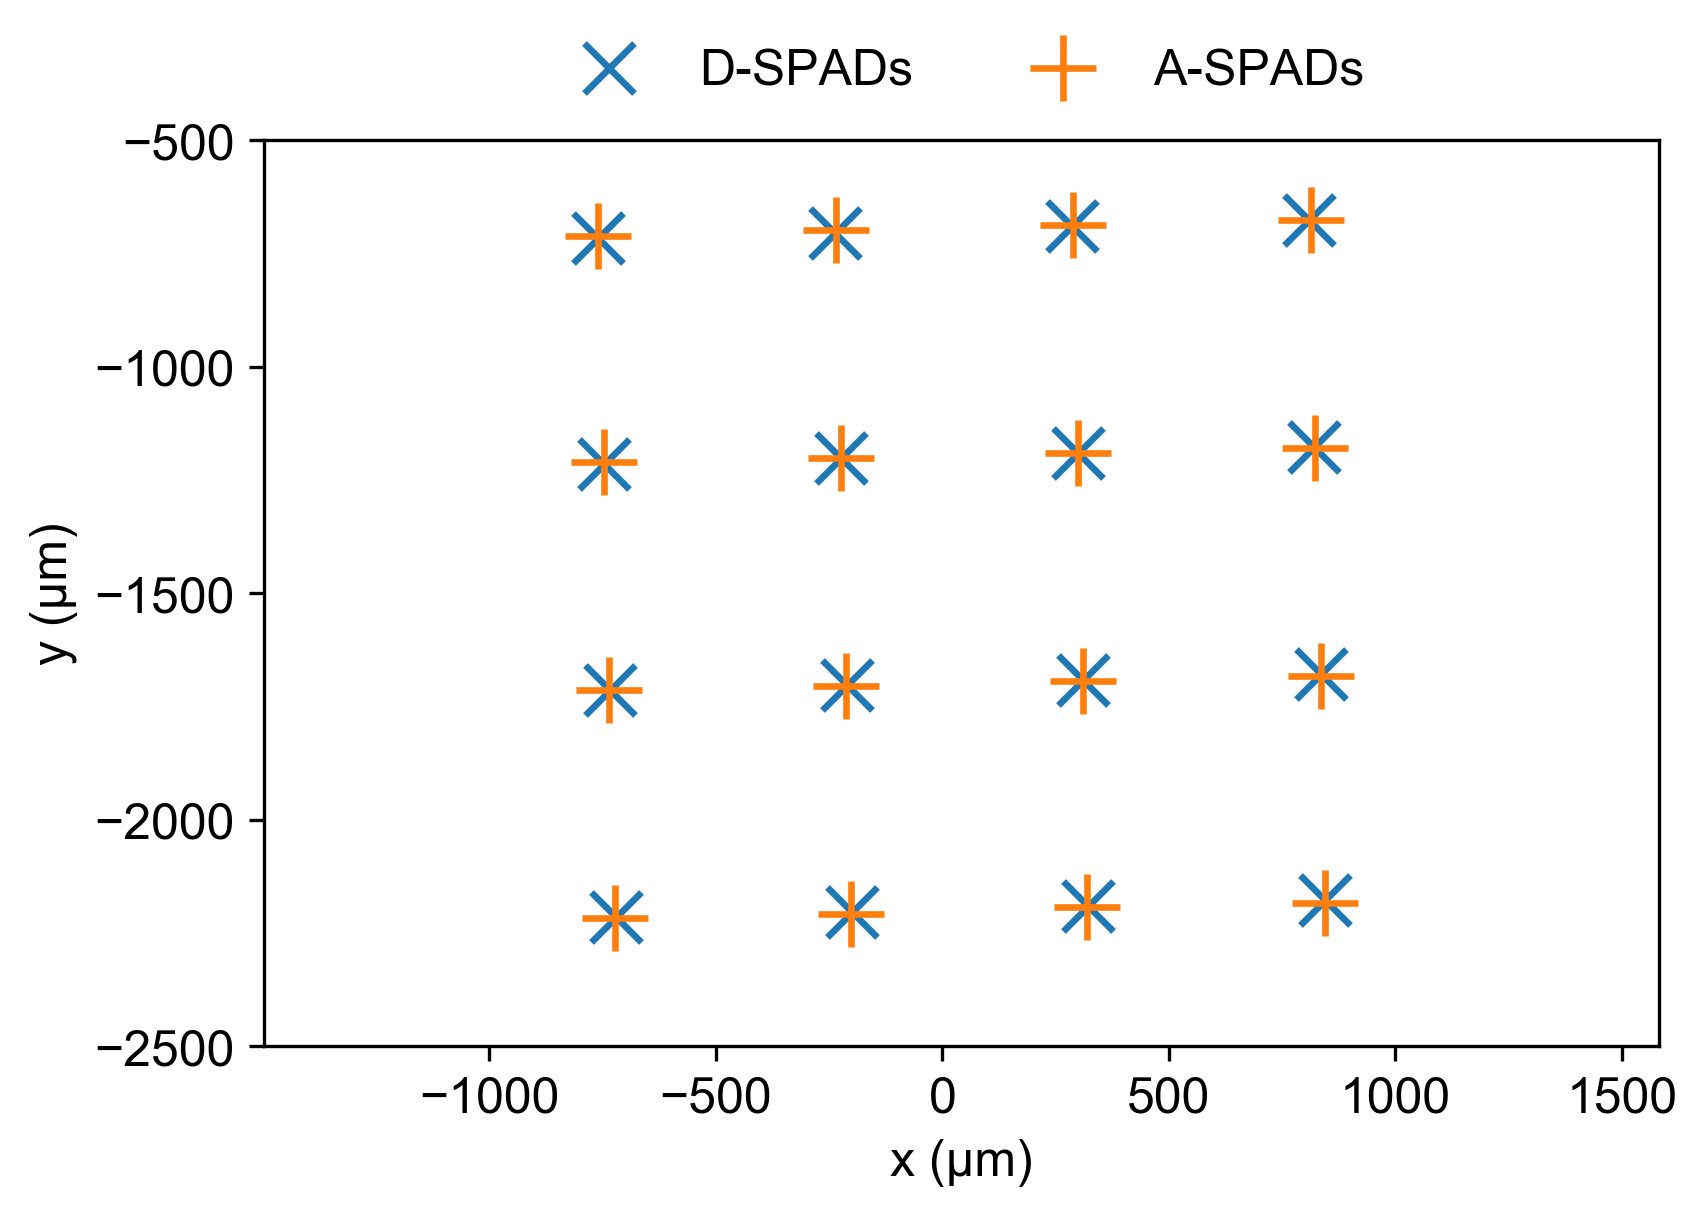
\includegraphics[width=\columnwidth]{figures/2017-05-02_scan_fit_scatter}
\caption{\label{fig:scatter-spad-align}
Experimental SPAD pixel coordinates after fine alignment for the D-SPAD
and A-SPAD arrays. D-SPAD denoted by
}
\end{figure*}

\section{ALEX and PAX}
\label{sec:alex_pax}

In ALEX, two alternation periods $D_{ex}$ and $A_{ex}$ (respectively D or A
excitation) and two detectors (D and A) are involved. This results in four
basic photon streams named $D_{ex}D_{em}$, $D_{ex}A_{em}$, $A_{ex}D_{em}$,
$A_{ex}A_{em}$, where the first symbol indicates the excitation period and the
second the detection channel. The $A_{ex}D_{em}$ stream only contains
background because there is no fluorescent emission in the D spectral band
during A-laser excitation. For simplicity, we assume here that these
quantities have been corrected for
background~\cite{ingargiola_fretbursts:_2016}.

A PAX setup has two detectors (D and A) but only one alternating laser (A). We
can still define two periods, one when only the D laser is on ($D_{ex}$) and
one when both lasers are on (${DA}_{ex}$). As in ALEX, combining the two
excitation periods and the two detectors leads to four basic PAX photon
streams: $D_{ex}D_{em}$, $D_{ex}A_{em}$, $DA_{ex}D_{em}$, $DA_{ex}A_{em}$.
Formally, the only difference with the ALEX photon stream is that $A_{ex}$ in
ALEX is replaced with $DA_{ex}$ in PAX. Differently from ALEX, however, all
four photon streams in PAX contain useful fluorescent signal. In particular,
$DA_{ex}D_{em}$ contains D fluorescence due to D laser excitation, while the
corresponding term $A_{ex}D_{em}$ in ALEX contains only background. With this
notation, in both ALEX and PAX, we can define the total fluorescence signal
during D excitation (e.g.~burst size):

\begin{equation}
    \Lambda = {F_{D_{ex}D_{em}} + F_{FRET}}
    \label{eq:burstsize_raw}
\end{equation}

\noindent where the $F$ quantities are background-corrected photon counts.
$F_{FRET}$ is the A fluorescence due to FRET, computed by
subtracting D-leakage and A-direct-excitation from $F_{D_{ex}A_{em}}$:

\begin{equation}
    F_{FRET} = F_{D_{ex}A_{em}} - Lk\,F_{D_{ex}D_{em}} - Dir
    \label{eq:F_FRET}
\end{equation}

We also need the usual correction factors $\gamma$ and
$\beta$~\cite{lee_accurate_2005}:

\begin{align}
    \gamma &= \frac{\phi_A \, \eta_{A_{det}}^{A_{em}}}
                   {\phi_D \, \eta_{D_{det}}^{D_{em}}} \label{eq:gamma} \\
    \beta &= \frac{I_{A_{ex}}\sigma_{A_{ex}}^A}{I_{D_{ex}}\sigma_{D_{ex}}^D}
    \label{eq:beta}
\end{align}

\noindent where $\phi_A$, $\phi_D$ are the dye quantum yields
and $\eta_{A_{det}}^{A_{em}}$, $\eta_{D_{det}}^{D_{em}}$ are the PDEs of the

D and A channels.
In eq.~\ref{eq:beta}, $I_{A_{ex}}$ and $I_{D_{ex}}$ are A and D excitation
intensities, while $\sigma_{A_{ex}}^A$ and $\sigma_{D_{ex}}^D$
are the dye absorption cross-sections at the respective laser wavelengths.
$\beta$ accounts for the difference of D and A dye fluorescence when
each dye is excited by its respective laser.

We can define the $\gamma$-corrected total signal
as~\cite{lee_accurate_2005,ingargiola_applying_2017}:

\begin{equation}
    \Lambda_\gamma = {\gamma\,F_{D_{ex}D_{em}} + F_{FRET}}
    \label{eq:burstsize}
\end{equation}

Differently from $\Lambda$, the quantity $\Lambda_\gamma$ does not change with
FRET (as long as the dyes quantum efficiency does not change).

With these definitions, we can write the expression for proximity ratio
$E_{PR}$ and FRET efficiency $E$ which is valid for both ALEX and PAX:

\begin{align}
    E_{PR} &= \frac{F_{FRET}}{\Lambda} \label{eq:Epr} \\
    E &= \frac{F_{FRET}}{\Lambda_\gamma} \label{eq:E}
\end{align}

Conversely, the $S$ expression is slightly different for ALEX and PAX. In
ALEX we define $S$ and the corrected version $S_{\gamma\beta}$ as:

\begin{align}
    S &= \frac{\Lambda}{\Lambda + F_{AexAem}} \label{eq:S} \\
    S_{\gamma\beta} &= \frac{\Lambda_\gamma}
                            {\Lambda_\gamma + \frac{F_{AexAem}}{\beta}}
                            \label{eq:Sgb}
\end{align}

The value $S_{\gamma\beta}$ is always centered around 0.5 for dual-labeled
species, regardless of FRET efficiency or D and A excitation intensities.

In PAX, we do not measure the $F_{A_{ex}A_{em}}$ directly, but we can
compute it as:

\begin{equation}
    \tilde{F}_{A_{ex}A_{em}} = F_{DA_{ex}A_{em}} - F_{D_{ex}A_{em}}
    \label{eq:pax_Faa}
\end{equation}

By replacing $F_{A_{ex}A_{em}}$ with $\tilde{F}_{A_{ex}A_{em}}$,
the PAX expressions for $S$ and $S_{\gamma\beta}$ become formally identical
to eq.~\ref{eq:S} and \ref{eq:Sgb}:

\begin{align}
S &= \frac{\Lambda}
          {\Lambda + \tilde{F}_{AexAem}} \label{eq:Spax} \\
S_{\gamma\beta} &= \frac{\Lambda_\gamma}
                        {\Lambda_\gamma + \frac{\tilde{F}_{AexAem}}{\beta}}
         \label{eq:Sgb_pax}
\end{align}

In PAX we can take advantage of the additional signal in
$F_{A_{ex}D_{em}}$ and derive an equivalent set of PAX-enhanced
expressions for $E$ and $S$. We can
start extending the definitions of the total FRET signal of
eq.~\ref{eq:burstsize_raw} and~\ref{eq:burstsize} by including
$F_{A_{ex}D_{em}}$ as follows:

\begin{align}
    \Lambda_{PAX} &= {F_{D_{ex}D_{em}} + F_{A_{ex}D_{em}} + 2 F_{FRET}}
    \label{eq:burstsizerawpaxe} \\
    \Lambda_{\gamma,PAX} &= {\gamma\,(F_{D_{ex}D_{em}} + F_{A_{ex}De_{m}}) + 2 F_{FRET}}
    \label{eq:burstsize_paxe}
\end{align}

Based on eq.~\ref{eq:burstsizerawpaxe} and \ref{eq:burstsize_paxe}, we
can write PAX-enhanced expressions for $E$ and $S$:

\begin{align}
    E_{PR,PAX} &= \frac{2\,F_{FRET}}{\Lambda_{PAX}} \label{eq:Epr_paxe} \\
    E_{PAX} &= \frac{2\,F_{FRET}}{\Lambda_{\gamma,PAX}} \label{eq:Epaxe} \\
    S_{PAX} &= \frac{\Lambda_{PAX}}{\Lambda_{PAX} + \tilde{F}_{A_{ex}A_{em}}}
    \label{eq:Spaxe} \\
    S_{\gamma\beta,PAX} &= \frac{\Lambda_{\gamma,PAX}}
        {\Lambda_{\gamma,PAX} + \frac{2\tilde{F}_{A_{ex}A_{em}}}{\beta}}
    \label{eq:Sgb_paxe}
\end{align}

Eq.~\ref{eq:Epr_paxe}, \ref{eq:Epaxe}, \ref{eq:Spaxe}
and~\ref{eq:Sgb_paxe} contain more photons than the classical expressions
and, therefore, can result in lower shot-noise. However, this effect is
mitigated by the fact that $F_{FRET}$ is counted twice (to
compensate for the doubling of the D signal) and, therefore, its
shot-noise is amplified.


\subsection{Modified stoichiometry}
\label{sec:Su}

By replacing $\tilde{F}_{A_{ex}A_{em}}$ with $F_{A_{ex}DA_{em}}$ in
eq.~\ref{eq:Spax}, we define the "modified stoichiometry" $S_u$
used in this paper as:

\begin{equation}
S_u = \frac{\Lambda}
{\Lambda + F_{A_{ex}DA_{em}}}
\label{eq:Su}
\end{equation}

This expression avoids the subtraction of photon counts
(and the corresponding increase in shot-noise) necessary in PAX to
compute $\tilde{F}_{A_{ex}A_{em}}$ (eq.~\ref{eq:pax_Faa}).
As a result, the
$S_u$ distributions are tighter, permitting easier
separation of FRET and D-only population. Note, however, that $S_u$ has a
built-in dependency on the population FRET value, in particular
$S_u$ decreases with the increasing $E$.
In this work, even at low FRET values, better separation between
FRET and D-only population was achieved using $S_u$ instead of
$S$. In general, the preference of $S_u$ over $S$ may change in
other PAX setups when the signal-to-noise and
background-to-noise ratios is significantly higher.
Once populations are separated, one
can return using the classical $S$ expression for the
purpose of computing gamma factors. Our interest, in the current paper,
was not recovering absolute FRET values and D-A distances, but rather
demonstrating the capabilities of the smFRET-PAX system in terms of
spot uniformity and throughput increase. Therefore, we did not compute a
complete gamma factor calibration. However, we addressed the differences
in collection and detection efficiency across the different spots using
a ``relative'' gamma coefficient $\chi_{ch}$ as illustrated in
section \ref{sec:perchcorr}.


\section{Individual channel corrections}
\label{sec:perchcorr}

\subsection{Gamma correction}

The gamma-factor of each channel, $\gamma_{ch}$, can be expressed as
the product of an average factor $\gamma_m$ and a spot-specific adjustment
factor $\chi_{ch}$:

\begin{equation}
\gamma_{ch} = \gamma_m \cdot \chi_{ch}
\label{eq:gamma_split}
\end{equation}

$\chi_{ch}$ can be easily computed from measurable
quantities according to the following expression:

\begin{equation}
\chi_{ch} = \frac{\frac{1}{\langle E_{PR\,ch} \rangle_{ch}} - 1}{\frac{1}{E_{PR\,ch}} - 1}
\label{eq:chich}
\end{equation}

In eq.~\ref{eq:chich}, $E_{PR\,ch}$ is the population-level
proximity ratio for a specific channel, and $ \langle E_{PRch} \rangle_{ch} $
is the average over all $N$ channels (in this case $N= 48$).

Eq.~\ref{eq:chich} follows from the following relation between $E$
and $E_{PR}$\cite{lee_accurate_2005, ingargiola_applying_2017}:

\begin{equation}
E = f(E_{PR}, \gamma) = \frac{1}{1 + \gamma \left( \frac{1}{E_{PR}} - 1 \right)}
\label{eq:EfuncEpr}
\end{equation}

Solving eq.~\ref{eq:EfuncEpr} for $\gamma$, we obtain:

\begin{equation}
\gamma = \frac{\frac{1}{E} - 1}{\frac{1}{E_{PR}} - 1}
\label{eq:gamma_funcEEpr}
\end{equation}

Formally, we can write $\gamma = \gamma_1 \gamma_2 $, where $\gamma_1$
is associated with a partially corrected
proximity ratio $E_1$ as follows:

\begin{equation}
E_1 = f(E_{PR}, \gamma_1) = \frac{1}{1 + \gamma_1 \left( \frac{1}{E_{PR}} - 1 \right)}
\label{eq:E1funcEpr}
\end{equation}

Writing $\gamma_1$ as a function of $E_1$ as in~\ref{eq:gamma_funcEEpr} and
substituting the expression into eq.~\ref{eq:EfuncEpr},
we obtain $E$ as a function of $E_{1}$:

\begin{equation}
E = f(E_1, \gamma_2) = \frac{1}{1 + \gamma_2 \left( \frac{1}{E_1} - 1 \right)}
\label{eq:EfuncE1}
\end{equation}

Eq.~\ref{eq:EfuncE1} has the same form as \ref{eq:EfuncEpr}
and~\ref{eq:EfuncE1}. Therefore,
$E$ can be obtained by two subsequent (chained) corrections for $\gamma_1$ and
$\gamma_2$ respectively as in eq.~\ref{eq:EfuncEprE1}.

\begin{equation}
E = f(E_{PR}, \gamma) =  f(E_1, \gamma_2) = f(f(E_{PR}, \gamma_1), \gamma_2)
\label{eq:EfuncEprE1}
\end{equation}

In the multispot case, we apply this property to decompose the gamma
correction into a spot-specific correction and an average correction as
in~\ref{eq:gamma_split}.
In particular, eq.~\ref{eq:chich} directly derives from~\ref{eq:gamma_funcEEpr}
with simple substitutions.

\subsection{Beta correction}

Since, formally eq.~\ref{eq:S} and~\ref{eq:Sgb} have the same form as
$E_{PR}$ and $E$, we can write an expression
equivalent to~\ref{eq:EfuncEpr} for $S$ and
$S_{\gamma\beta}$. Dropping the $\gamma$ subscript, we
obtain:

\begin{equation}
S_{\beta} = \frac{1}{1 + \frac{1}{\beta} \left( \frac{1}{S} - 1 \right)}
\label{eq:SbfuncS}
\end{equation}

Following the same arguments as in the previous section,
the beta correction can be expressed as the product of a spot-average
$\beta_m$ and an individual channel correction $\beta_{ch}$:

\begin{equation}
\beta = \beta_m \, \beta_{ch}
\label{eq:beta_factor}
\end{equation}

Similarly to eq.~\ref{eq:chich}, we can compute $\beta_{ch}$ as:

\begin{equation}
\frac{1}{\beta_{ch}} = \frac{\frac{1}{\langle S_{ch} \rangle_{ch}} - 1}{\frac{1}{S_{ch}} - 1}
\label{eq:betach}
\end{equation}

\noindent where $S_{ch}$ is the population-level non-beta-corrected
stoichiometry  ratio for a specific channel, and $ \langle S_{ch} \rangle_{ch} $ is the
average over all $N$
channels ($N= 48$ in this case).

\section{Additional data}
\label{sec:moredata}

Fig.~\ref{fig:alexhist48all22d} shows $E_{PR}$-$S_u$ histograms for the
different channels obtained during the measurement of a 22d DNA sample
(low-FRET). Due to the choice of donor and acceptor excitation powers
during this measurement, the FRET population has an $S_u$ value larger
than 0.5, artificially compressing the histograms in the upper part of
the graphs. Nonetheless, it is still possible to distinguish FRET from
D-only bursts, despite the low value of $E_{PR}$ for that sample, allowing
a bias-free estimation of $E_{PR}$, as opposed to what would have happened
in the absence of acceptor excitation~\cite{ingargiola_multispot_2017}.

\begin{figure*}
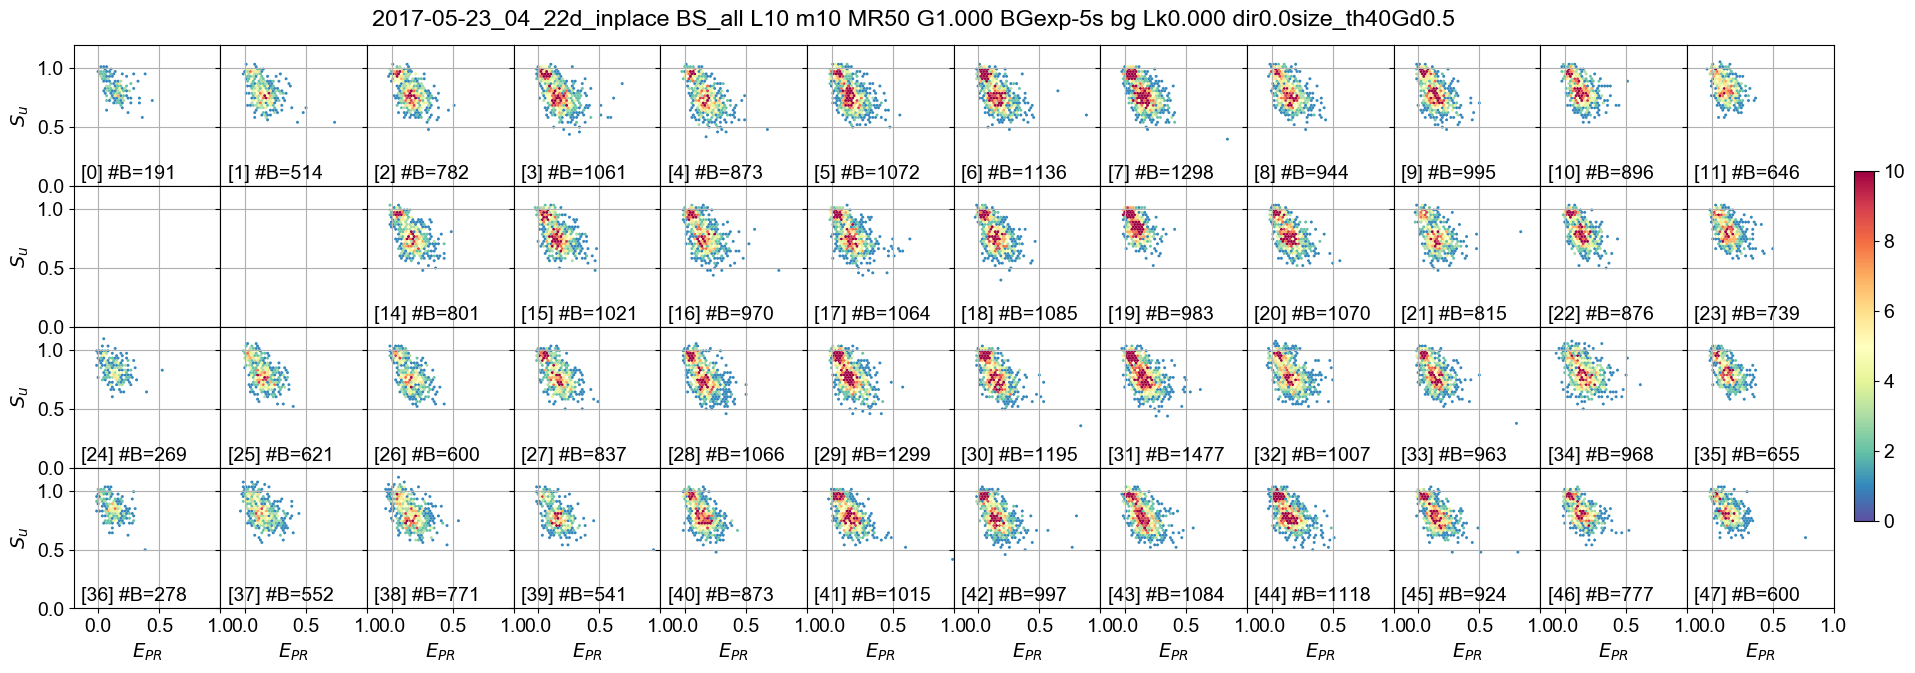
\includegraphics[width=\textwidth]{figures/2017-05-23_04_22d_48spot_alex_hist_Su_all-bursts}
\caption{{\label{fig:alexhist48all22d} $E_{PR}$ versus $S_u$
histograms of all spots for the 22d dsDNA sample. Data analysis and
burst search are identical as in figure~\ref{fig:alexhist48all12d}.
Burst search was performed using all photons with
constant-threshold burst search (50~kcps). Burst selection was performed
on the total burst size after background correction, using a threshold of
40 photons. The legend in each subplot
reports spot number ($[\cdot]$) and number of bursts (\#B).%
}}
\end{figure*}

\nocite{*}
\bibliography{biblio}% Produces the bibliography via BibTeX.

\end{document}
%
% ****** End of file aipsamp.tex ******
